\chapter[Desenvolvimento do Projeto]{Desenvolvimento do Projeto}

O capítulo apresenta o projeto realizado nesta dissertação, contendo a explicação do que foi desenvolvido, os circuitos esquemáticos, os parâmetros dos componentes e os layouts dos blocos desenvolvidos. Alguns circuitos não foram incluídos neste capítulo e são apresentados de maneira implícita, devido à sua simplicidade, flexibilidade de implementação em replicações do trabalho, e devido o autor também entender que os mesmos já são de amplo conhecimento na área. No \autoref{blocosadicionais} é possível verificar mais sobre esses blocos e como foram desenvolvidos, caso o leitor sinta a necessidade de entender a sua implementação.

Ao longo de todo capítulo, tabelas serão apresentadas com as seguintes identificações

\begin{itemize}
\item $W$ é a largura do canal (transistor) ou largura do componente (resistor e diodo) [${\mu}m$]
\item $L$ é a comprimento do canal (transistor) ou comprimento do componente (resistor e diodo) [${\mu}m$]
\item $M$ é o número de dispositivos em paralelo [$n$°$ dispositivos$]
\item $S$ é o número de dispositivos em série [$n$°$ dispositivos$]
\end{itemize}

\newcommand{\NomeBloco}{NULL}
\newcommand{\NomeBlocoNoIt}{NULL}
\newcommand{\NomeBlocoNoUnderline}{NULL}
\newcommand{\NomePTab}{tab_\NomeBlocoNoUnderline}
\newcommand{\NomeSTab}{tab_\NomeBlocoNoUnderline2}
\newcommand{\NomePFig}{fig_\NomeBlocoNoUnderline}
\newcommand{\NomeSFig}{fig_\NomeBlocoNoUnderline2}
\newcommand{\NomeTTab}{tab_\NomeBlocoNoUnderline3}
\newcommand{\NomeQTab}{tab_\NomeBlocoNoUnderline4}

\section[Projeto de um Receptor Óptico]{Projeto de um Receptor Óptico}
\label{sec_circ_comp}

Um circuito integrado foi desenvolvido para a comunicação de dados via luz, utilizando-se dos circuitos apresentados na \autoref{section:APS} e \autoref{section:TIA} deste documento. O projeto \'e representado em alto n\'ivel na \autoref{fig_circcompleto}. A \autoref{fig_circcompletohigh} mostra uma representação dos principais blocos presentes no circuito.

Todos os sinais aqui apresentados na figura, e tamb\'em em todas figuras \`a seguir, seguem o padrão descrito na \autoref{section:padrao_sinais} deste trabalho.

A tensão de alimentação utilizada em todos os blocos do projeto apresentado é de \textit{1.8 V}, e é representada pelo nome \textit{VDD}.

\begin{figure}[!h]
    	\caption{\label{fig_circcompleto}Optoreceptor projetado}
	\begin{center}
	    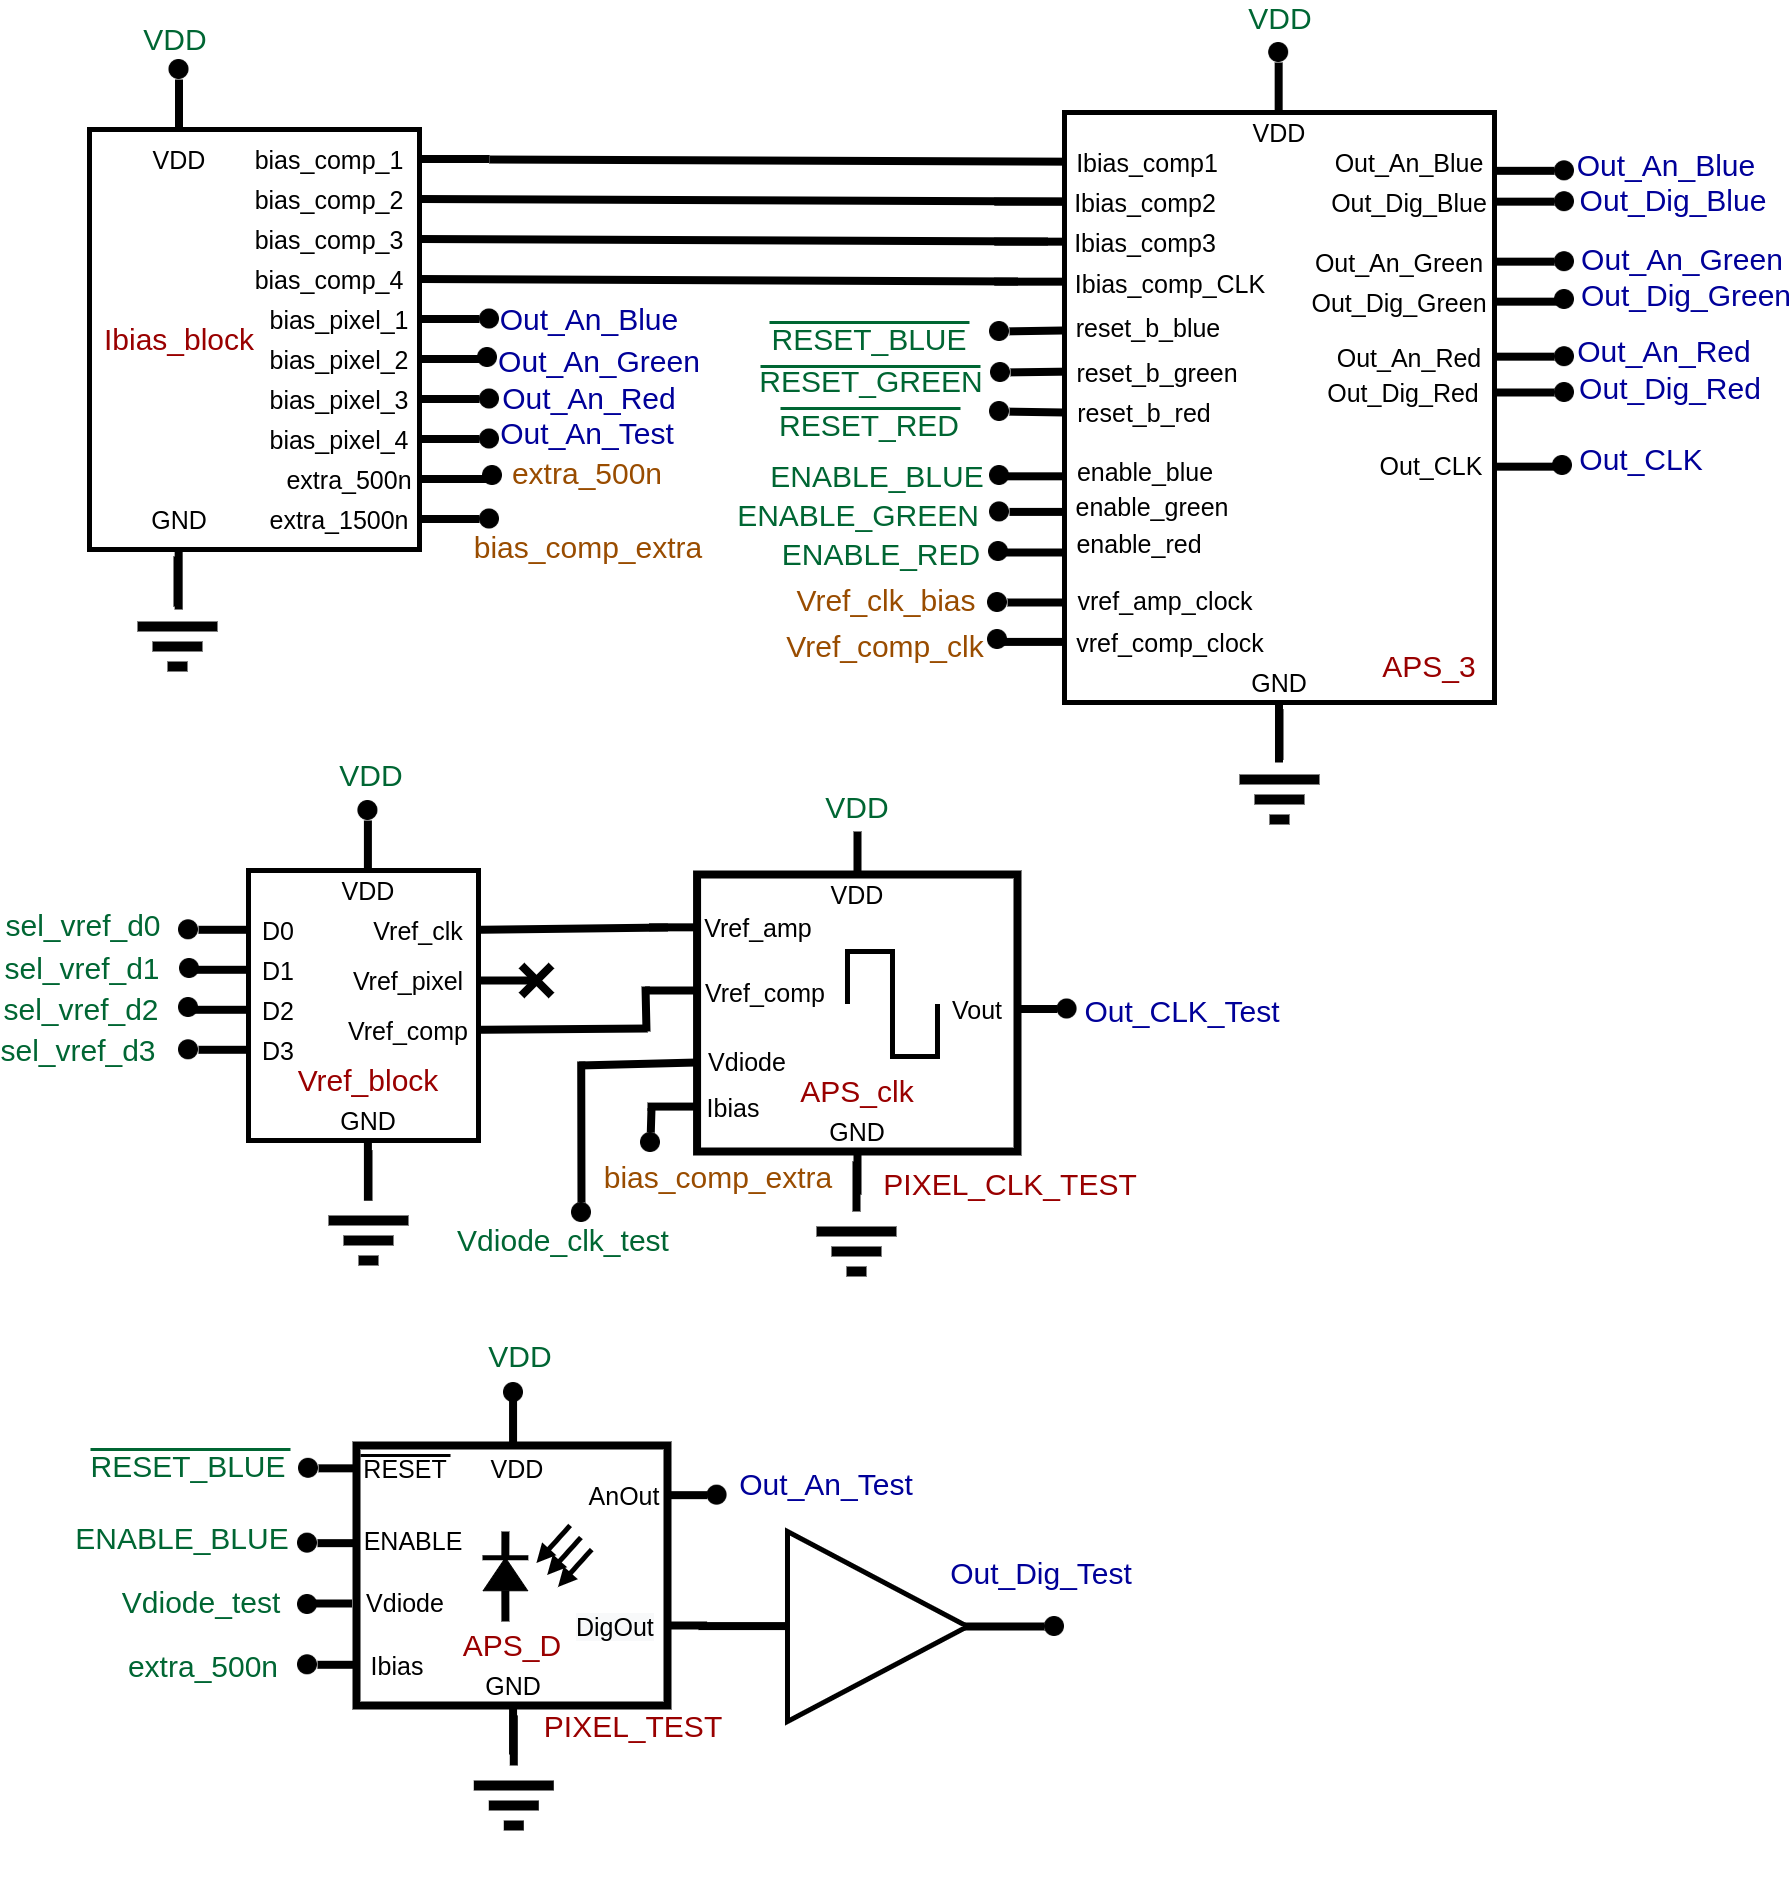
\includegraphics[width=\textwidth]{Circuitos/Complete_Circuit.png}
	\end{center}
	\legend{Fonte: Produzido pelo autor}
\end{figure}

\begin{figure}[!h]
	\caption{\label{fig_circcompletohigh}Representação dos principais blocos presentes no projeto}
	\begin{center}
	    \includegraphics[width=\textwidth]{Imagens/Complete_Circuit_rep.png}
	\end{center}
	\legend{Fonte: Produzido pelo autor}
\end{figure}


O circuito tem a finalidade de processar a informação advinda de tr\^es APS's, constru\'idos de maneira id\^entica em n\'ivel de layout, com a finalidade de abstrair informações de cores advindas de uma fonte luminosa, dos quais podem ser Azul, Verde ou Vermelha. Para que as cores fossem devidamente separadas, são utilizadas películas coloridas externas, que ficam acima de cada respectivo circuito APS de forma a permitir passar somente a informação de uma cor.

Um sinal luminoso de cor branca tamb\'em \'e utilizado no sistema de forma a ser a refer\^encia de rel\'ogio de todos APS's descritos. Esse sinal \'e processado utilizando-se um TIA, do qual \'e gerado um sinal el\'etrico equivalente \`a informação luminosa.

A tecnologia de fabricação utilizada para o desenvolvimento de todos blocos foi a \textit{CMOS TSMC 180nm}. O software utilizado para o projeto do dispositivo foi o \textit{Virtuoso}, desenvolvido pela empresa \textit{Cadence}.

O circuito representado na \autoref{fig_circcompleto} \'e composto por 2 blocos principais, que permitem o processamento advindos da fonte luminosa, al\'em de um circuito APS e um TIA extra. A descrição dos bloco são:

\begin{itemize}
    \item \textit{ibias\_block}: Tem a função de gerar fontes de corrente utilizadas em alguns blocos do circuito.
    
    \item \textit{APS\_3}: Implementa os tr\^es circuitos \textit{APS} descritos, al\'em do circuito TIA. A sa\'ida de cada bloco passa por um comparador de forma a digitalizar o dado, como ser\'a melhor explicitado na \autoref{sec_apsdigitalized}.
    
    \item \textit{Vref\_block} e \textit{PIXEL\_CLK\_TEST}: Estes blocos realizam a implementação de um TIA, por\'em com a adição de um pino extra que possibilita a simulação de uma corrente fotogerada sem necessitar de uma fonte luminosa. Estes blocos serão melhor explicados na \autoref{BlocoTestes}. 
    
    \item \textit{PIXEL\_TEST}: Este bloco realiza a implementação de um APS, com a adição de um pino adicional onde pode ser injetado uma corrente sem a necessidade de uma fonte luminosa. Este bloco será melhor explicado na \autoref{BlocoTestes}.
    
\end{itemize}

A \autoref{tab_circcomp2} mostra a relação de sinais de entrada e sa\'ida presentes no circuito para o processamento dos blocos de teste. A \autoref{tab_circcomp} mostra a relação de sinais de entrada e sa\'ida presentes no circuito, para o processamento dos p\'ixels de cor.

\begin{table}[ht]
  \caption{Descrição dos sinais de entrada e sa\'ida do circuito projetado para os blocos de teste}%
  \label{tab_circcomp2}
  \begin{tabular}{ccl}
  \toprule
   Sinal & Tipo & Descrição \\
   \midrule \midrule
   Vdiode\_test & Entrada & Corrente que simula um potencial no fotodiodo do APS de teste\\
   \midrule
   Vdiode\_clk\_test & Entrada & Corrente que simula um potencial no fotodiodo no TIA de teste\\
   \midrule
   Out\_An\_Test & Sa\'ida & Sinal de tensão anal\'ogico para o APS de teste \\
   \midrule
   Out\_Dig\_Test & Sa\'ida & Sinal de tensão digital para o APS de teste \\
  \midrule
   Out\_CLK\_test & Sa\'ida & Sinal de tensão de rel\'ogio gerado pelo TIA de teste\\
  \bottomrule
\end{tabular}%
  \legend{Fonte: Produzido pelo autor.}
\end{table}

\begin{table}[!h]
\centering
\caption{\label{tab_circcomp}Descrição dos sinais de entrada e sa\'ida do circuito projetado para as cores azul, verde e vermelha}%
  \begin{tabular}{ccll}
  \toprule
   Sinal & Tipo & Descrição & Observação \\
  \midrule \midrule
   RESET\_BLUE & Entrada & \begin{tabular}[l]{@{}l@{}}Sinal de tensão de \textit{RESET}\\ no APS para cor azul\end{tabular}   & Ativo em n\'ivel baixo \\
  \midrule
   RESET\_GREEN & Entrada & \begin{tabular}[l]{@{}l@{}}Sinal de tensão de \textit{RESET}\\ no APS  para cor verde\end{tabular}   & Ativo em n\'ivel baixo \\
  \midrule
   RESET\_RED & Entrada & \begin{tabular}[l]{@{}l@{}}Sinal de tensão de \textit{RESET}\\ no APS  para cor vermelha\end{tabular}   & Ativo em n\'ivel baixo \\
  \midrule
   ENABLE\_BLUE & Entrada & \begin{tabular}[l]{@{}l@{}}Sinal de tensão de \textit{ENABLE}\\ no APS para cor azul\end{tabular}   & Ativo em n\'ivel alto \\
  \midrule
   ENABLE\_GREEN & Entrada & \begin{tabular}[l]{@{}l@{}}Sinal de tensão de \textit{ENABLE}\\ no APS para cor verde\end{tabular}   & Ativo em n\'ivel alto \\
  \midrule
   ENABLE\_RED & Entrada & \begin{tabular}[l]{@{}l@{}}Sinal de tensão de \textit{ENABLE}\\ no APS para cor vermelha\end{tabular}   & Ativo em n\'ivel alto \\
  \midrule
   Out\_An\_Blue & Sa\'ida & \begin{tabular}[l]{@{}l@{}}Sinal de tensão anal\'ogica\\ para cor azul\end{tabular} \\
  \midrule
   Out\_Dig\_Blue & Sa\'ida & \begin{tabular}[l]{@{}l@{}}Sinal de tensão digital\\ para cor azul\end{tabular} \\
  \midrule
   Out\_An\_Green & Sa\'ida & \begin{tabular}[l]{@{}l@{}}Sinal de tensão anal\'ogica\\ para cor verde\end{tabular} \\
  \midrule
   Out\_Dig\_Green & Sa\'ida & \begin{tabular}[l]{@{}l@{}}Sinal de tensão digital\\ para cor verde\end{tabular} \\
  \midrule
   Out\_An\_Red & Sa\'ida & \begin{tabular}[l]{@{}l@{}}Sinal de tensão anal\'ogica\\ para cor vermelha\end{tabular} \\
  \midrule
   Out\_Dig\_Red & Sa\'ida & \begin{tabular}[l]{@{}l@{}}Sinal de tensão digital\\ para cor vermelha\end{tabular} \\
   \midrule
   Out\_CLK & Sa\'ida & \begin{tabular}[l]{@{}l@{}}Sinal de tensão de rel\'ogio\\ gerado pelo TIA\end{tabular}\\
  \bottomrule
\end{tabular}%

\legend{Fonte: Produzido pelo autor.}
\end{table}

\section{Espelhos de Corrente}

Espelhos de Corrente foram necess\'arios para o desenvolvimento de diversos blocos contidos no projeto, e serão especificados nas subseções seguintes. Uma explicação geral sobre o funcionamento e desenvolvimento de espelhos de corrente pode ser vista no \autoref{anexoespelhos}.

\renewcommand{\NomeBloco}{\textit{ibias\_generator}}
\renewcommand{\NomeBlocoNoUnderline}{ibiasgenerator}
\renewcommand{\NomePTab}{tab_\NomeBlocoNoUnderline}
\renewcommand{\NomeSTab}{tab_\NomeBlocoNoUnderline2}
\renewcommand{\NomePFig}{fig_\NomeBlocoNoUnderline}
\renewcommand{\NomeSFig}{fig_\NomeBlocoNoUnderline2}
\renewcommand{\NomeTTab}{tab_\NomeBlocoNoUnderline3}
\renewcommand{\NomeQTab}{tab_\NomeBlocoNoUnderline4}

\subsection{ibias\_generator}
 
O bloco \NomeBloco{}\footnote{Circuito desenvolvido pelo aluno \textit{Daniel Carvalho Lott}, do curso de bacharelado em Engenharia Elétrica da UFMG, no ano de 2020} \'e um espelho de corrente que apresenta uma sa\'ida de 50 $\mu$A. O bloco apresenta as definições de sinais de entrada e sa\'ida referidos na \autoref{\NomeSTab}.

\begin{table}[!h]
\caption{Sinais do bloco \NomeBloco}
\label{\NomeSTab}
\centering
\begin{tabular}{ccl}

    \toprule
    Sinal & Tipo    & Descrição        \\
    \midrule \midrule
    ibias\_1   & Saída   & Fonte de Corrente de 50 $\mu$A \\
    \bottomrule
\end{tabular}
\legend{Fonte: Produzido pelo autor}
\end{table}

O circuito projetado para o bloco \'e demonstrado na \autoref{\NomePFig}.

\begin{figure}[htb]
 \centering
    \centering
    \caption{Circuito CMOS projetado para o bloco \NomeBloco} 
    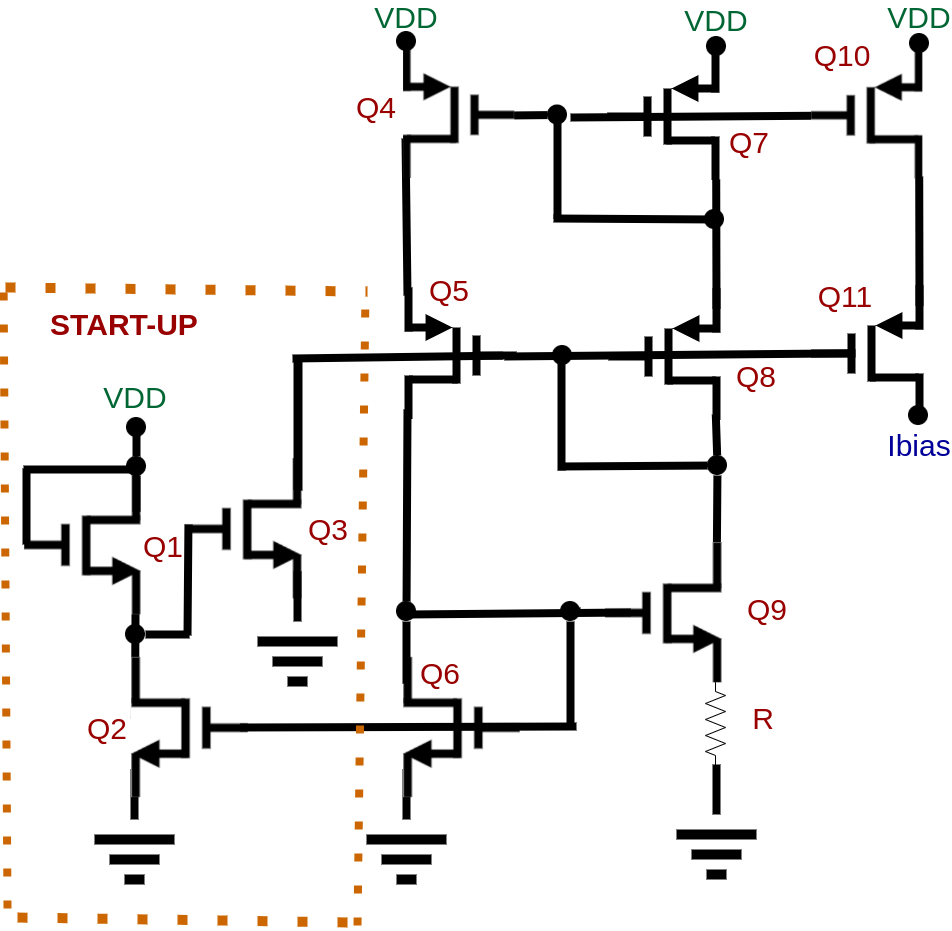
\includegraphics[scale=0.3]{Circuitos/Ibias_generator.png}
    \legend{Fonte: Produzido pelo autor}
    \label{\NomePFig}
\end{figure}

\begin{figure}[htb]
 \centering
    \centering
    \caption{\label{\NomeSFig}Representação em bloco do \NomeBloco}
    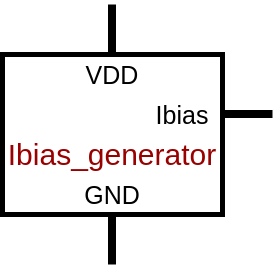
\includegraphics[scale=0.3]{Circuitos/ibias_generator_block.png}
    \legend{Fonte: Produzido pelo autor}
\end{figure}

Os transistores utilizados no bloco apresentam os par\^ametros mostrados na \autoref{\NomeTTab}.

\begin{table}[!h]
\caption{Transistores do Bloco \NomeBloco}
\label{\NomeTTab}
\centering
\begin{tabular}{ccccc}
\toprule
Transistor & W ($\mu$m)  & L ($\mu$m)           & M (n° dispositivos) & S (n° dispositivos)\\
\midrule \midrule
Q1 & 0,3 & 19,995 & 1 & 3\\
\midrule
Q2 & 25 & 0,5 & 2 & 1\\
\midrule
Q3 & 30 & 0,5 & 1 & 1\\
\midrule
Q4, Q7 e Q10 & 35 & 4 & 2 & 1\\
\midrule
Q5, Q8 e Q11 & 25 & 2,5 & 2 & 1\\
\midrule
Q6 & 20 & 4 & 2 & 1\\
\midrule
Q9 & 20 & 4 & 4 & 1\\
\midrule
Q10 & 25 & 2,5 & 2 & 1\\
\midrule
Q11 & 25 & 2,5 & 2 & 1\\
\bottomrule
\end{tabular}
\legend{Fonte: Produzido pelo autor}
\end{table}

O resistor utilizado no bloco apresenta os par\^ametros mostrados na \autoref{\NomeQTab}.

\begin{table}[!h]
\caption{Resistor do bloco \NomeBloco}
\label{\NomeQTab}
\centering
\begin{tabular}{ccccc}
\toprule
Resistor & W ($\mu$m)  & L ($\mu$m) & M (n° dispositivos) & Resist\^encia (k$\Omega$)\\
\midrule \midrule
R & 8 & 29,98 & 2 & 0,569025\\
\bottomrule
\end{tabular}
\legend{Fonte: Produzido pelo autor}
\end{table}

Os transistores \textit{Q6} e \textit{Q9}, juntos aos resistores \textit{R1} e \textit{R2}, t\^em a finalidade de funcionarem como um dreno de corrente referenciados pelos resistores. Os transistores \textit{Q4} e \textit{Q7} t\^em a finalidade de funcionarem como uma fonte de corrente, referenciados pelo dreno de corrente j\'a mencionado. O transistor \textit{Q10} \'e o braço do espelho de corrente do qual fornece a corrente de sa\'ida.

Os transistores \textit{Q5}, \textit{Q8} e \textit{Q11} se apresentam na configuração \textit{Cascode}, que tem o intuito de tornar o espelho de corrente de resposta mais linear, aumentar sua banda e ainda aumentar as suas resist\^encias de entrada e sa\'ida.

Os transistores \textit{Q1}, \textit{Q2} e \textit{Q3} t\^em a função de inicializar o circuito no ponto de operação adequado, j\'a que o circuito tamb\'em apresenta estabilidade quando fornecendo 0 A, sendo necess\'ario evitar essa situação que pode acontecer no momento que o circuito é ligado, estando inicialmente em 0 V.

\renewcommand{\NomeBloco}{\textit{iref\_generator}}
\renewcommand{\NomeBlocoNoUnderline}{irefgenerator}
\renewcommand{\NomePTab}{tab_\NomeBlocoNoUnderline}
\renewcommand{\NomeSTab}{tab_\NomeBlocoNoUnderline2}
\renewcommand{\NomePFig}{fig_\NomeBlocoNoUnderline}
\renewcommand{\NomeSFig}{fig_\NomeBlocoNoUnderline2}
\renewcommand{\NomeTTab}{tab_\NomeBlocoNoUnderline3}
\renewcommand{\NomeQTab}{tab_\NomeBlocoNoUnderline4}

\subsection{iref\_generator}

O bloco \NomeBloco{}\footnote{Circuito desenvolvido por \textit{Dalton Martini Colombo}, orientador do trabalho aqui apresentado} \'e um espelho de corrente que apresenta algumas sa\'idas como fonte e outras em dreno de corrente. O bloco apresenta as definições de sa\'ida referidos na \autoref{\NomeSTab}.

\begin{table}[!h]
\caption{Sinais do bloco \NomeBloco}
\label{\NomeSTab}
\centering
\begin{tabular}{ccl}

    \toprule
    Sinal & Tipo    & Descrição        \\
    \midrule \midrule
    iref1\_src   & Saída   & Fonte de Corrente de 0.5 $\mu$A \\
    \midrule
    iref2\_src   & Saída   & Fonte de Corrente de 0.5 $\mu$A \\
    \midrule
    iout\_test   & Saída   & Fonte de Corrente de 1.5 $\mu$A \\
    \midrule
    iref1\_sink   & Saída   & Dreno de Corrente de 0.5 $\mu$A \\
    \midrule
    iref2\_sink   & Saída   & Dreno de Corrente de 0.5 $\mu$A \\
    \bottomrule
\end{tabular}
\legend{Fonte: Produzido pelo autor}
\end{table}

O circuito projetado para o bloco \'e demonstrado na \autoref{\NomePFig}.

\begin{figure}[htb]
 \centering
    \centering
    \caption{Circuito CMOS projetado para o bloco \NomeBloco} 
    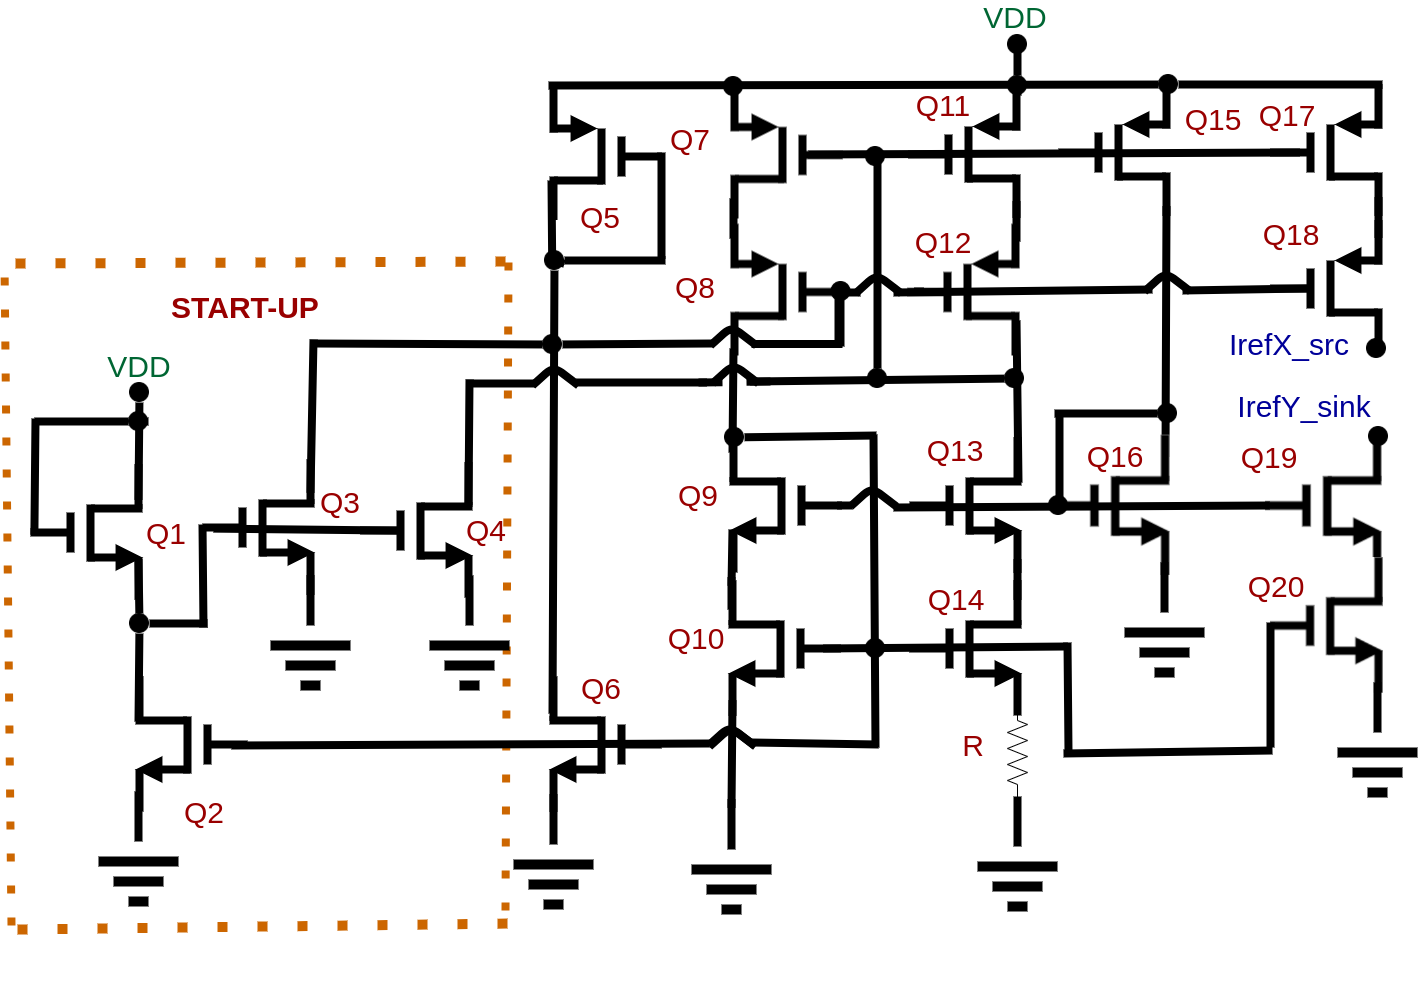
\includegraphics[scale=0.3]{Circuitos/iref_generator.png}
    \legend{Fonte: Produzido pelo autor}
    \nota{Nem todos transistores são representados na imagem. \emph{Q17}, \emph{Q18}, \emph{Q19} e \emph{Q20} são transistores replicados para cada sa\'ida \emph{IrefX\_src} e \emph{IrefY\_sink}, onde \emph{X} e \emph{Y} são os identificadores de cada sa\'ida}
    \label{\NomePFig}
\end{figure}

\begin{figure}[htb]
 \centering
    \centering
    \caption{\label{\NomeSFig}Representação em bloco do \NomeBloco}
    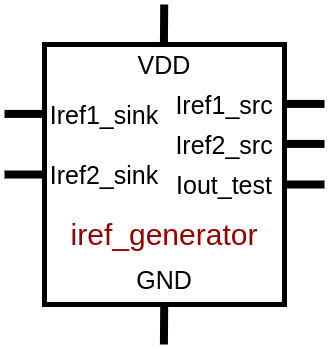
\includegraphics[scale=0.3]{Circuitos/iref_generator_block.png}
    \legend{Fonte: Produzido pelo autor}
\end{figure}

Os transistores utilizados no bloco apresentam os par\^ametros mostrados na \autoref{\NomeTTab}.

\begin{table}[!h]
\caption{Transistores do Bloco \NomeBloco}
\label{\NomeTTab}
\centering
\begin{tabular}{ccccc}
\toprule
Transistor & W ($\mu$m)  & L ($\mu$m)  & M (n° dispositivos) & S (n° dispositivos)\\
\midrule \midrule

\midrule
Q1                                   & 0,3    & 19,995 & 1                   & 3                   \\
\midrule
Q2                                   & 35     & 0,18   & 2                   & 1                   \\
\midrule
Q3 e Q4                              & 15     & 0,18   & 1                   & 1                   \\
\midrule
Q5                                   & 10     & 15     & 1                   & 6                   \\
\midrule
\begin{tabular}[c]{@{}c@{}}Q6, Q9, Q10,\\ Q13, Q19 e Q20\end{tabular}          & 4      & 19,995 & 1                   & 2                   \\
\midrule
\begin{tabular}[c]{@{}c@{}}Q7, Q8, Q11, Q12,\\ Q15, Q17a¹ e Q18a¹\end{tabular} & 10     & 15   & 2                   & 1                   \\
\midrule
Q14                                  & 4      & 19,995 & 10                  & 1                   \\
\midrule
Q16                                  & 4      & 19,995 & 1                   & 6 \\
\midrule
Q17b² e Q18b²                                                                  & 10     & 15     & 6                   & 1                  \\
\bottomrule
\end{tabular}
\legend{Fonte: Produzido pelo autor}
\legend{¹ Q17a e Q18a são os transistores referentes \`as sa\'idas iref1\_src e iref2\_src\\
² Q17b e Q18b são os transistores referentes \`a sa\'ida iout\_test}
\end{table}

O resistor \emph{R} utilizado no bloco apresenta os par\^ametros mostrado na \autoref{\NomeQTab}.

\begin{table}[!h]
\caption{Resistor do bloco \NomeBloco}
\label{\NomeQTab}
\centering
\begin{tabular}{cccc}
\toprule
Resistor & W ($\mu$m)  & L ($\mu$m) & Resist\^encia (k$\Omega$)\\
\midrule \midrule
R & 3 & 404,4 & 141,996\\
\bottomrule
\end{tabular}
\legend{Fonte: Produzido pelo autor}
\end{table}

Os transistores \emph{Q6} e \emph{Q9}, juntos ao resistor R, t\^em a finalidade de funcionarem como um dreno de corrente referenciados pelo resistor. Os transistores \emph{Q4} e \emph{Q7} t\^em a finalidade de funcionarem como uma fonte de corrente, referenciados pelo dreno de corrente j\'a mencionado. O transistor \emph{Q10} \'e o braço do espelho de corrente do qual fornece a corrente de sa\'ida.

Os transistores \emph{Q5}, \emph{Q8} e \emph{Q11} se apresentam na configuração \emph{Cascode}, que tem o intuito de tornar o espelho de corrente de resposta mais linear, aumentar sua banda e ainda aumentar as suas resist\^encias de entrada e sa\'ida.

Os transistores \emph{Q1}, \emph{Q2} e \emph{Q3} t\^em a função de inicializarem o circuito no ponto de operação adequado, j\'a que o circuito tamb\'em apresenta estabilidade quando fornecendo 0 A, sendo necess\'ario evitar essa situação.

\renewcommand{\NomeBloco}{\textit{current\_mirror\_nmos}}
\renewcommand{\NomeBlocoNoUnderline}{curmirnmosb}
\renewcommand{\NomePTab}{tab_\NomeBlocoNoUnderline}
\renewcommand{\NomeSTab}{tab_\NomeBlocoNoUnderline2}
\renewcommand{\NomePFig}{fig_\NomeBlocoNoUnderline}
\renewcommand{\NomeSFig}{fig_\NomeBlocoNoUnderline2}
\renewcommand{\NomeTTab}{tab_\NomeBlocoNoUnderline3}
\renewcommand{\NomeQTab}{tab_\NomeBlocoNoUnderline4}

\subsection{current\_mirror\_nmos}

O bloco \NomeBloco{} cont\'em alguns braços utilizados como dreno de corrente para outras partes do circuito, sendo todos valores iguais \`a corrente de refer\^encia. O bloco apresenta as definições de sinais de entrada e sa\'ida referidos na \autoref{\NomeSTab}.

\begin{table}[!h]
\caption{Sinais do bloco \NomeBloco}
\label{\NomeSTab}
\centering
\begin{tabular}{ccl}

    \toprule
    Sinal & Tipo    & Descrição        \\
    \midrule \midrule
    Iref\_bias   & Entrada   &  Corrente de refer\^encia para os braços \\
    \midrule
    Iref\_A   & Saída   &  Braço 1 \\
    \midrule
    Iref\_B   & Saída   &  Braço 2 \\
    \midrule
    Iref\_C   & Saída   &  Braço 3 \\
    \midrule
    Iref\_D   & Saída   &  Braço 4 \\
    \midrule
    Iref\_E   & Saída   &  Braço 5 \\
    \bottomrule
\end{tabular}
\legend{Fonte: Produzido pelo autor}
\end{table}

O circuito projetado para o bloco \'e demonstrado na \autoref{\NomePFig}.

\begin{figure}[htb]
 \centering
    \centering
    \caption{Circuito CMOS projetado para o bloco \NomeBloco} 
    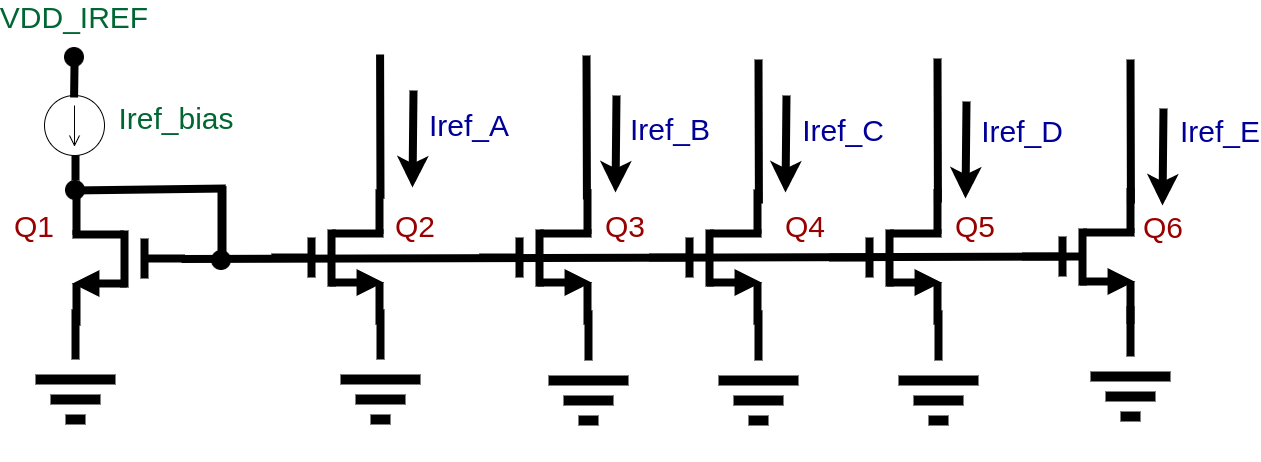
\includegraphics[scale=0.3]{Circuitos/current_mirror.png}
    \legend{Fonte: Produzido pelo autor}
    \label{\NomePFig}
\end{figure}

\begin{figure}[htb]
 \centering
    \centering
    \caption{\label{\NomeSFig}Representação em bloco do \NomeBloco} 
    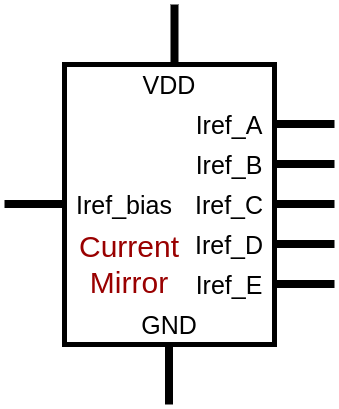
\includegraphics[scale=0.3]{Circuitos/current_mirror_block.png}
    \legend{Fonte: Produzido pelo autor}
\end{figure}

Os transistores utilizados no bloco apresentam os par\^ametros mostrados na \autoref{\NomeTTab}.

\begin{table}[!h]
\caption{Transistores do Bloco \NomeBloco}
\label{\NomeTTab}
\centering
\begin{tabular}{ccccc}
\toprule
Transistor & W ($\mu$m)  & L ($\mu$m)           & M (n° dispositivos) & S (n° dispositivos)\\
\midrule \midrule
\begin{tabular}[c]{@{}c@{}}Q1, Q2, Q3,\\
Q4, Q5 e Q6\end{tabular} & 5 & 6 & 2 & 1\\
\bottomrule
\end{tabular}
\legend{Fonte: Produzido pelo autor}
\end{table}
\renewcommand{\NomeBloco}{\textit{APS}}
\renewcommand{\NomeBlocoNoUnderline}{blocoAPS}
\renewcommand{\NomePTab}{tab_\NomeBlocoNoUnderline}
\renewcommand{\NomeSTab}{tab_\NomeBlocoNoUnderline2}
\renewcommand{\NomePFig}{fig_\NomeBlocoNoUnderline}
\renewcommand{\NomeSFig}{fig_\NomeBlocoNoUnderline2}
\renewcommand{\NomeTTab}{tab_\NomeBlocoNoUnderline3}
\renewcommand{\NomeQTab}{tab_\NomeBlocoNoUnderline4}

\section{APS}

O bloco \NomeBloco{} implementa o circuito apresentado na \autoref{fig_APS}. O bloco apresenta as definições de sinais de entrada e sa\'ida referidos na \autoref{\NomeSTab}.

\begin{table}[!h]
\label{\NomeSTab}
\begin{tabular}{ccll}
\toprule
Sinal      & Tipo    & \multicolumn{1}{c}{Descrição}                                                          & \multicolumn{1}{c}{Observação}                                                                               \\
\midrule \midrule
RESET      & Entrada & Sinal de tensão de RESET no APS                                                        & Ativo em nível baixo                                                                                         \\
\midrule
ENABLE     & Entrada & Sinal de tensão de ENABLE no APS                                                       & Ativo em nível alto                                                                                          \\
\midrule
SELECT     & Entrada & Sinal de tensão de SELECT no APS                                                       & \begin{tabular}[c]{@{}l@{}}Ativo em nível alto.\\ Mantido internamente \\ em nível alto\end{tabular} \\
\midrule
Ibias\_clk & Entrada & Dreno de Corrente do bloco (500 nA)                                                    &                                                                                                              \\
\midrule
Vout       & Saída   & \begin{tabular}[c]{@{}l@{}}Sinal de tensão analógica produzido\\ pelo APS\end{tabular} &    \\
\bottomrule
\end{tabular}
\legend{Fonte: Produzido pelo autor.}
\end{table}

A representação em bloco do circuito projetado é dado na \autoref{\NomeSFig}.

\begin{figure}[!h]
 \centering
    \centering
    \caption{\label{\NomeSFig}Representação em bloco do \NomeBloco} 
    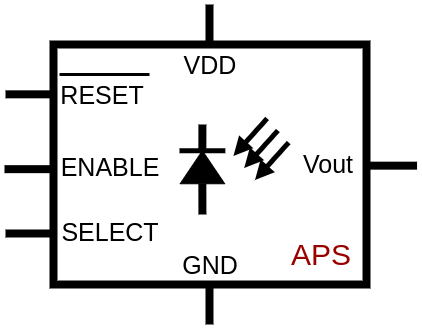
\includegraphics[scale=0.3]{Circuitos/APS_block.png}
    \legend{Fonte: Produzido pelo autor}
\end{figure}

Os transistores utilizados no bloco apresentam os par\^ametros mostrados na \autoref{\NomeTTab}.

\begin{table}[!h]
\caption{Transistores do bloco \NomeBloco}
\label{\NomeTTab}
\centering
\begin{tabular}{ccccc}
\toprule
Transistor & W ($\mu$m)  & L ($\mu$m)           & M (n° dispositivos) & S (n° dispositivos)\\
\midrule \midrule
T\textsubscript{buffer} & 15 & 0,75 & 1 & 1\\
\midrule
T\textsubscript{reset} & 4 & 0,18 & 1 & 1\\
\midrule
T\textsubscript{select} & 10 & 0,18 & 2 & 2\\
\bottomrule
\end{tabular}
\legend{Fonte: Produzido pelo autor}
\end{table}

O fotodiodo utilizado no bloco apresenta os par\^ametros mostrados na \autoref{\NomeQTab}. $W$ é a largura do fotodiodo. $L$ é o comprimento do fotodiodo.

\begin{table}[!h]
\caption{Fotodiodo do bloco \NomeBloco}
\label{\NomeQTab}
\centering
\begin{tabular}{cccc}
\toprule
Nome & W ($\mu$m)  & L ($\mu$m) & Área ($\mu$m²)\\
\midrule \midrule
Fotodiodo & 25 & 25 & 625\\
\bottomrule
\end{tabular}
\legend{Fonte: Produzido pelo autor}
\end{table}

Informações referentes à $T\textsubscript{enable}$ podem ser vistas no \autoref{portatg}.
\renewcommand{\NomeBloco}{\textit{APS\_digitalized}}
\renewcommand{\NomeBlocoNoUnderline}{apsdigitalized}
\renewcommand{\NomePTab}{tab_\NomeBlocoNoUnderline}
\renewcommand{\NomeSTab}{tab_\NomeBlocoNoUnderline2}
\renewcommand{\NomePFig}{fig_\NomeBlocoNoUnderline}
\renewcommand{\NomeSFig}{fig_\NomeBlocoNoUnderline2}
\renewcommand{\NomeTTab}{tab_\NomeBlocoNoUnderline3}
\renewcommand{\NomeQTab}{tab_\NomeBlocoNoUnderline4}

\section{APS\_digitalized}
\label{sec_apsdigitalized}

O \textit{APS\_digitalized} \'e o circuito respons\'avel por digitalizar o sinal gerado pelo APS descrito na \autoref{section:APS}. O bloco apresenta as definições de sinais de entrada e sa\'ida referidos na \autoref{\NomeSTab}.

\begin{table}[!h]
\caption{Sinais do bloco \NomeBloco}
\label{\NomeSTab}
\centering
\begin{tabular}{ccll}

    \toprule
    Sinal & Tipo    & Descrição & Observação        \\
    \midrule \midrule
    RESET   & Entrada   & Sinal de tensão de RESET no APS & Ativo em nível baixo\\
    \midrule
    ENABLE   & Entrada   & Sinal de tensão de ENABLE no APS & Ativo em nível alto\\
    \midrule
    Vref   & Entrada   & \begin{tabular}[l]{@{}l@{}}Tensão de refer\^encia utilizada pelo\\ \textit{Comparador}\end{tabular} \\
    \midrule
    Ibias   & Entrada   & Corrente de polarização do comparador \\
    \midrule
    AnOut   & Saída   & \begin{tabular}[l]{@{}l@{}}Sinal de tensão anal\'ogica produzido\\ pelo APS\end{tabular} \\
    \midrule
    DigOut   & Saída   & \begin{tabular}[l]{@{}l@{}}Sinal de tensão digital produzido\\ pelo \textit{Comparador}\end{tabular} \\
    \bottomrule
\end{tabular}
\legend{Fonte: Produzido pelo autor}
\end{table}

O circuito projetado para o bloco \'e demonstrado nas figuras \ref{repblocoAPS} e \ref{repblocoAPS2}.

\begin{figure}[!h]
 \centering
    \centering
    \caption{Circuito CMOS projetado para o bloco \NomeBloco com o circuito do APS explicito} 
    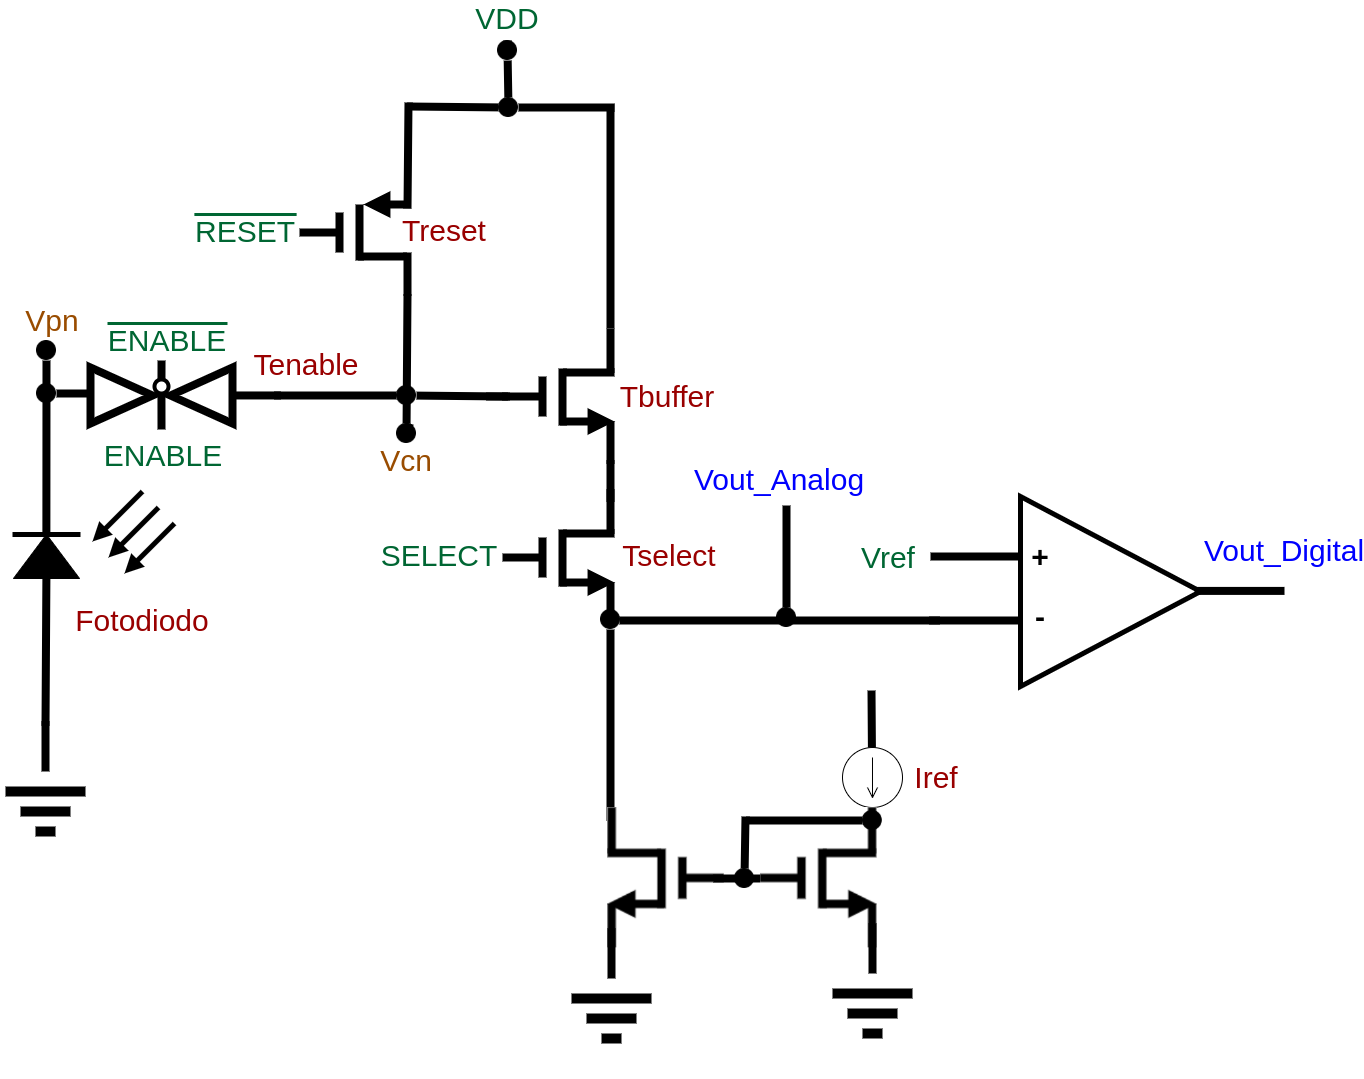
\includegraphics[scale=0.3]{Circuitos/APS_digitalized_rep.png}
    \legend{Fonte: Produzido pelo autor}
    \label{repblocoAPS}
\end{figure}

\begin{figure}[!h]
 \centering
    \centering
    \caption{Circuito CMOS projetado para o bloco \NomeBloco} 
    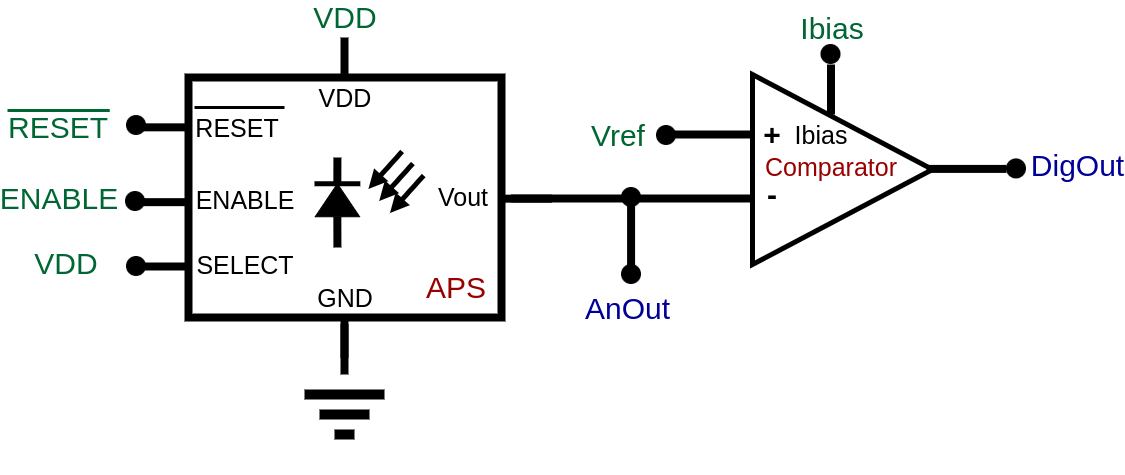
\includegraphics[scale=0.3]{Circuitos/APS_digitalized.png}
    \legend{Fonte: Produzido pelo autor}
    \label{repblocoAPS2}
\end{figure}

\begin{figure}[!h]
 \centering
    \centering
    \caption{\label{\NomeSFig}Representação em bloco do \NomeBloco}
    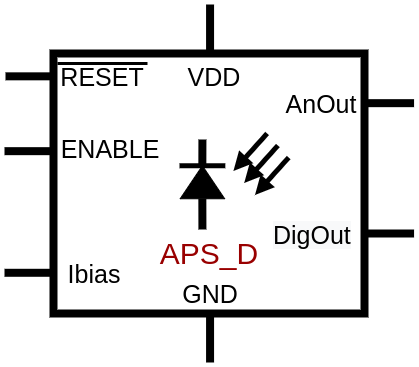
\includegraphics[scale=0.3]{Circuitos/APS_digitalized_block.png}
    \legend{Fonte: Produzido pelo autor}
\end{figure}

A sa\'ida digital do bloco funciona realizando uma comparação entre uma tensão de refer\^encia chamada de \textit{Vref} e a sa\'ida anal\'ogica do APS, chamada de \textit{AnOut}. Quando o valor de \textit{Vref} for maior do que o de \textit{AnOut}, o comparador ir\'a saturar e apresentar um sinal aproximadamente igual a VDD, interpretada como n\'ivel l\'ogico '1'. Quando o valor de \textit{Vref} for menor ou igual do que o de \textit{AnOut}, o comparador ir\'a apresentar um sinal aproximadamente igual a GND em sua sa\'ida, interpretada como n\'ivel l\'ogico '0'.

Utilizando o elemento comparador, podemos ajustar para que a sa\'ida retorne '0' apenas quando for atingido um valor limiar controlado. Como sabemos que a intensidade da corrente fotogerada depende da intensidade da luz captada pelo fotodiodo (\autoref{secao_fotodiodo}), podemos deduzir a informação sobre intensidade luminosa verificando em quanto tempo demora para que se mude de n\'ivel l\'ogico '1' para '0' durante o Est\'agio 2, considerando que o nó $V_{cn}$ apresentava o valor de VDD, que equivale à $AnOut$ apresentar o máximo valor em sua saída (\autoref{eq_voutfinal}). Considerando o atraso no comparador nulo, e desprezando-se as resistências das chaves no bloco APS, podemos utilizar as equações \ref{eq_responsividade}, \ref{eq_modEletFotIl} e \ref{eq_voutfinal} para se obter a \autoref{eq_apsd}.

\begin{equation}
    \label{eq_apsd}
    P_{FD} = \frac{(AnOut_0-V_{ref})(C_{j}+C_{cn})}{R_{\lambda}t_{1-0}}
\end{equation}

Onde:

\begin{itemize}

    \item \textit{P$_{FD}$} \'e a pot\^encia \'optica presente no fotodiodo [\textit{W}]
    \item $AnOut_0$ \'e o valor do nó $AnOut$ no momento que inicia o Período de Integração [$V$]
    \item \textit{$V_{ref}$} \'e a tensão de refer\^encia do comparador [$V$]
    \item \textit{$C_j$} \'e a capacit\^ancia de junção do fotodiodo [\textit{F}]
    \item \textit{$C_{cn}$} \'e a capacit\^ancia do n\'o central do APS [\textit{F}]
    \item $R_{\lambda}$ \'e a responsividade para o comprimento de onda detectado no fotodiodo [$A.W^{-1}$]
    \item $t_{1\_0}$ \'e o tempo do qual o n\'ivel l\'ogico demorou para mudar de '1' para '0', a partir do momento que se inicia o Estágio 2, representado na \autoref{figurataps}, equivalente ao tempo para que a tensão de saída do APS seja igual a Vref [\textit{s}]
    
\end{itemize}

\begin{figure}[!h]
 \centering
    \centering
    \caption{\label{figurataps}Comparação da saída do APS com a tensão de referência do comparador do $APS\_digitalized$ \NomeBloco} 
    \includegraphics[scale=0.3]{Imagens/Graficot.png}
    \legend{Fonte: Produzido pelo autor}
    \label{\NomePFig}
\end{figure}

\renewcommand{\NomeBloco}{\textit{APS\_pixel\_clk}}
\renewcommand{\NomeBlocoNoUnderline}{apspixelclk}
\renewcommand{\NomePTab}{tab_\NomeBlocoNoUnderline}
\renewcommand{\NomeSTab}{tab_\NomeBlocoNoUnderline2}
\renewcommand{\NomePFig}{fig_\NomeBlocoNoUnderline}
\renewcommand{\NomeSFig}{fig_\NomeBlocoNoUnderline2}
\renewcommand{\NomeTTab}{tab_\NomeBlocoNoUnderline3}
\renewcommand{\NomeQTab}{tab_\NomeBlocoNoUnderline4}

\section{APS\_pixel\_clk}

O \NomeBloco{}\footnote{Circuito esquemático desenvolvido por \textit{Dalton Martini Colombo}} \'e o bloco respons\'avel por processar e digitalizar o sinal gerado pelo \textit{TIA}. A intenção de uso do \textit{TIA} \'e que ele seja o respons\'avel por captar um sinal luminoso com frequ\^encia bem definida, e o sinal el\'etrico gerado, em forma de pulsos quadrados, sirva de refer\^encia de rel\'ogio para todos os circuitos APS utilizados para detecção de cor. O bloco portanto tem como responsabilidade gerar um sinal digital de frequ\^encia igual a do sinal luminoso captado. O bloco apresenta as definições de sinais de entrada e sa\'ida referidos na \autoref{\NomeSTab}.

\begin{table}[!h]
\caption{Sinais do bloco \NomeBloco}
\label{\NomeSTab}
\centering
\begin{tabular}{cclc}

    \toprule
    Sinal & Tipo    & Descrição  & Observação\\
    \midrule \midrule
    Vref\_comp   & Entrada   & Tensão de refer\^encia utilizada pelo comparador &  1,15 V\\
    \midrule
    Vref\_amp   & Entrada   & Tensão de refer\^encia utilizada para o TIA &  0,77 V\\
    \midrule
    Ibias   & Entrada   & Corrente de polarização do comparador & 500 nA \\
    \midrule
    Vout   & Saída   & Sinal digital produzido pelo Comparador\\
    \bottomrule
\end{tabular}
\legend{Fonte: Produzido pelo autor}
\end{table}

A \autoref{TIAsimplifC} mostra o circuito projetado de maneira simplificada. O circuito completo projetado para o bloco \'e demonstrado na \autoref{\NomePFig}.

\begin{figure}[!h]
 \centering
    \centering
    \caption{Circuito CMOS simplificado projetado para o bloco \NomeBloco} 
    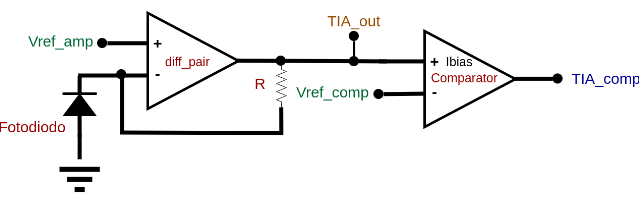
\includegraphics[scale=0.6]{Circuitos/TIA_ref.png}
    \label{TIAsimplifC}
    \legend{Fonte: Produzido pelo autor}
\end{figure}

\begin{figure}[!h]
 \centering
    \centering
    \caption{Circuito CMOS projetado para o bloco \NomeBloco} 
    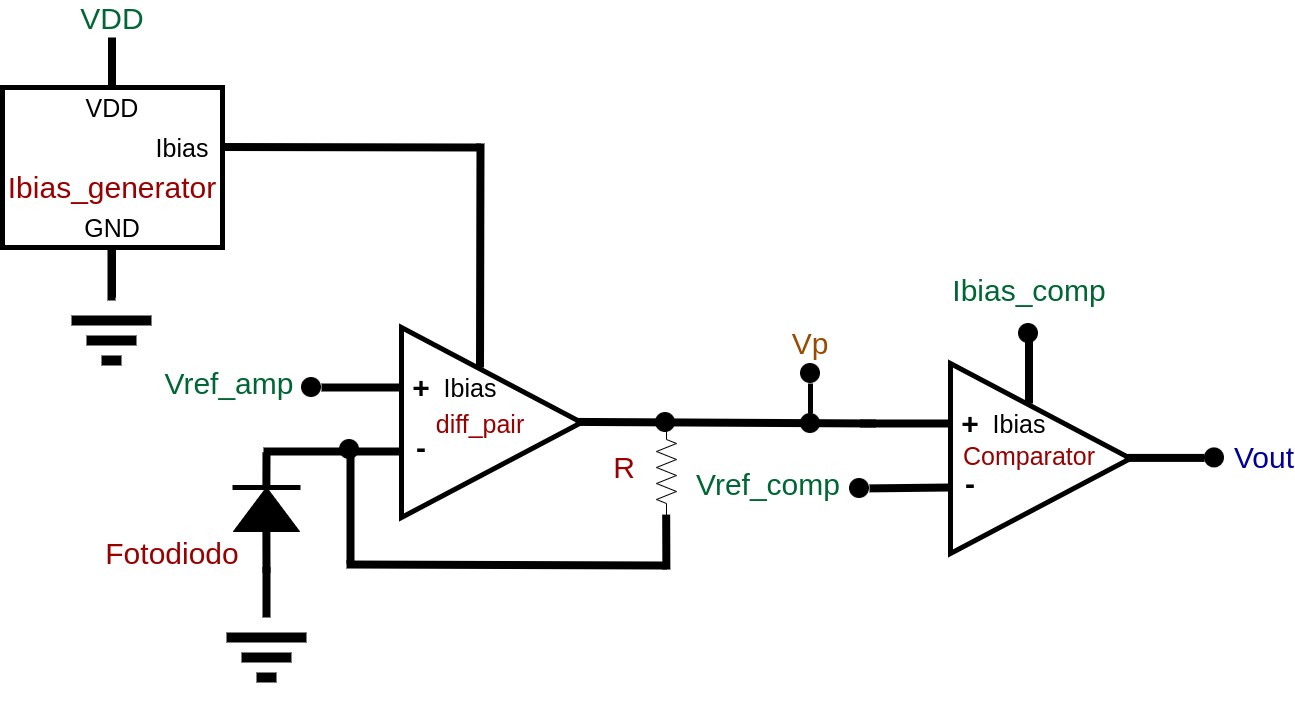
\includegraphics[scale=0.3]{Circuitos/APS_clk.png}
    \label{\NomePFig}
    \legend{Fonte: Produzido pelo autor}
\end{figure}

\begin{figure}[!h]
 \centering
    \centering
    \caption{\label{\NomeSFig}Representação em bloco do \NomeBloco}
    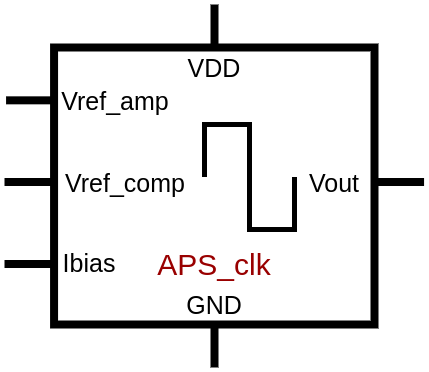
\includegraphics[scale=0.3]{Circuitos/APS_clk_block.png}
    \legend{Fonte: Produzido pelo autor}
\end{figure}

O circuito tem funcionamento similar ao do apresentado no bloco \textit{APS\_digitalized}, por\'em com apenas a sa\'ida digital sendo considerada e sendo utilizado um $TIA$ ao inv\'es de um \textit{APS}. A corrente de polarização do par diferencial \'e gerada pelo bloco \textit{Ibias\_generator}, contido no bloco.

Uma resist\^encia $R$ de ganho \'e utilizada, com valor apresentado na \autoref{\NomeQTab}. $W$ é a largura do resistor. $L$ é o comprimento do resistor.

\begin{table}[!h]
\caption{Resistor do bloco \NomeBloco}
\label{\NomeQTab}
\centering
\begin{tabular}{cccc}
\toprule
Resistor & W ($\mu$m)  & L ($\mu$m) & Resist\^encia (M$\Omega$)\\
\midrule \midrule
R & 1,68 & 39486,3 & 25\\
\bottomrule
\end{tabular}
\legend{Fonte: Produzido pelo autor}
\end{table}

O fotodiodo utilizado no bloco apresenta os par\^ametros mostrados na \autoref{\NomeTTab}. $W$ é a largura do fotodiodo. $L$ é o comprimento do fotodiodo.

\begin{table}[!h]
\caption{Fotodiodo do bloco \NomeBloco}
\label{\NomeTTab}
\centering
\begin{tabular}{cccc}
\toprule
Nome & W ($\mu$m)  & L ($\mu$m) & Área ($\mu$m²)\\
\midrule \midrule
Fotodiodo & 25 & 25 & 625\\
\bottomrule
\end{tabular}
\legend{Fonte: Produzido pelo autor}
\end{table}

Com base na \autoref{eqCTIA2}, a \autoref{eq_TIAblock} descreve $V_{p}$, que \'e comparada com \textit{Vref\_comp} e então utilizada para gerar o sinal de sa\'ida.

\begin{equation}
    \label{eq_TIAblock}
    V_{p} = RI_{PH}
\end{equation}

Onde:

\begin{itemize}

    \item \textit{$V_{P}$} \'e a tensão no ramo positivo do comparador [$V$]
    \item \textit{$I_{PH}$} \'e a corrente fotogerada [$A$]
    
\end{itemize}
\renewcommand{\NomeBloco}{\textit{vref\_generator}}
\renewcommand{\NomeBlocoNoUnderline}{vrefgenerator}
\renewcommand{\NomePTab}{tab_\NomeBlocoNoUnderline}
\renewcommand{\NomeSTab}{tab_\NomeBlocoNoUnderline2}
\renewcommand{\NomePFig}{fig_\NomeBlocoNoUnderline}
\renewcommand{\NomeSFig}{fig_\NomeBlocoNoUnderline2}
\renewcommand{\NomeTTab}{tab_\NomeBlocoNoUnderline3}
\renewcommand{\NomeQTab}{tab_\NomeBlocoNoUnderline4}

\section{vref\_generator}

O \textit{\NomeBloco}\footnote{Circuito esquemático desenvolvido por \textit{Dalton Martini Colombo}} \'e o bloco respons\'avel por gerar todas as tensões de refer\^encia utilizados nos outros blocos do circuito. O bloco apresenta as definições de sinais de entrada e sa\'ida referidos na \autoref{\NomeSTab}.

\begin{table}[!h]
\caption{Sinais do bloco \NomeBloco}
\label{\NomeSTab}
\centering
\begin{tabular}{ccl}

    \toprule
    Sinal & Tipo    & Descrição      \\
    \midrule \midrule
    Ibias   & Entrada   & Corrente de polarização do bloco \textit{Par Diferencial} \\
    \midrule
    V\_extra   & Saída   & Tensão de refer\^encia de 1,15 V \\
    \midrule
    Vref\_plus   & Saída   & Tensão de refer\^encia de 1,02 V \\
    \midrule
    Vref   & Saída   & Tensão de refer\^encia de 898,45 mV \\
    \midrule
    y1   & Saída   & Tensão de refer\^encia de 772,67 mV \\
    \midrule
    y2   & Saída   & Tensão de refer\^encia de 646,89 mV \\
    \midrule
    y3   & Saída   & Tensão de refer\^encia de 521,1 mV \\
    \midrule
    y4  & Saída   & Tensão de refer\^encia de 395,32 mV  \\
    \midrule
    y5   & Saída   & Tensão de refer\^encia de 269,54 mV \\
    \midrule
    y6   & Saída   & Tensão de refer\^encia de 143,75 mV \\
    \bottomrule
\end{tabular}
\legend{Fonte: Produzido pelo autor}
\end{table}

O circuito projetado para o bloco \'e demonstrado na \autoref{\NomePFig}.

\begin{figure}[htb]
 \centering
    \centering
    \caption{\label{\NomePFig}Circuito CMOS projetado para o bloco \NomeBloco} 
    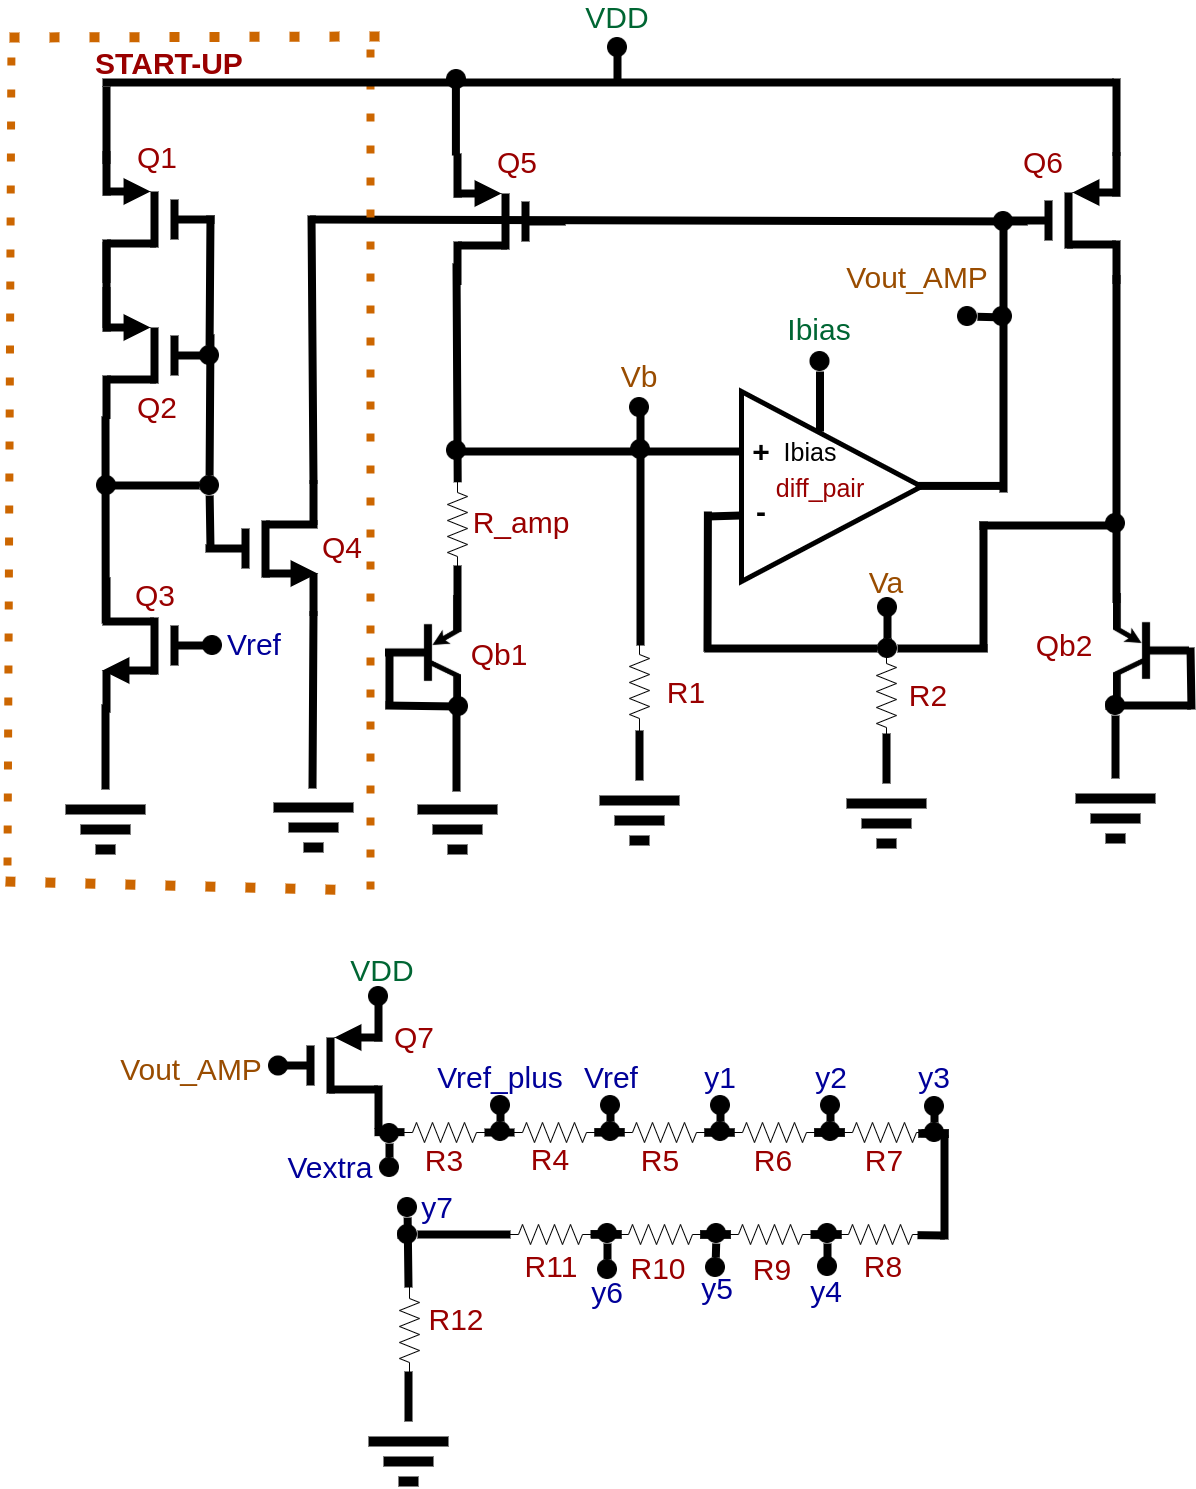
\includegraphics[scale=0.3]{Circuitos/vref_generator.png}
    \legend{Fonte: Produzido pelo autor}
\end{figure}

\begin{figure}[htb]
 \centering
    \centering
    \caption{\label{\NomeSFig}Representação em bloco do \NomeBloco}
    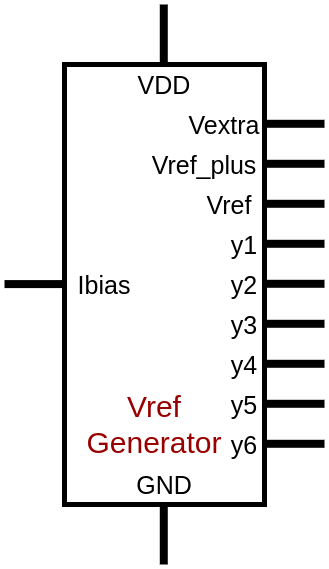
\includegraphics[scale=0.3]{Circuitos/vref_generator_block.png}
    \legend{Fonte: Produzido pelo autor}
\end{figure}

Os transistores utilizados no bloco \NomeBloco{} apresentam os par\^ametros mostrados na \autoref{\NomeTTab}.

\begin{table}[!h]
\caption{Transistores do Bloco \NomeBloco}
\label{\NomeTTab}
\centering
\begin{tabular}{ccccc}
\toprule
Transistor & W ($\mu$m)  & L ($\mu$m)           & M (n° dispositivos) & S (n° dispositivos)\\
\midrule \midrule
Q1 e Q2 & 0,5 & 19,995 & 1 & 1\\
\midrule
Q3 & 20 & 0,18 & 1 & 1\\
\midrule
Q4 & 2 & 0,18 & 1 & 1\\
\midrule
Q5, Q6 e Q7 & 20 & 16 & 4 & 1\\
\midrule
Qb1 (PNP) & 5 & 5 & 1 & 1\\
\midrule
Qb2 (PNP) & 5 & 5 & 8 & 1\\
\bottomrule
\end{tabular}
\legend{Fonte: Produzido pelo autor}
\end{table}

Os resistores utilizados no bloco \NomeBloco{} apresentam os par\^ametros mostrados na \autoref{\NomeQTab}.

\begin{table}[!h]
\caption{Resistores do bloco \NomeBloco}
\label{\NomeQTab}
\centering
\begin{tabular}{cccccc}
\toprule
Resistor & \begin{tabular}[c]{@{}c@{}}W \\($\mu$m)\end{tabular}   & \begin{tabular}[c]{@{}c@{}}L \\($\mu$m)\end{tabular}  & \begin{tabular}[c]{@{}c@{}}Resist\^encia\\ (k$\Omega$)\end{tabular} & \begin{tabular}[c]{@{}c@{}}M\\(n° dispositivos)\end{tabular} & \begin{tabular}[c]{@{}c@{}}S \\(n° dispositivos)\end{tabular}\\
\midrule \midrule
R1 e R2 & 2 & 18,85 & 10,1024 & 1 & 10\\
\midrule
\begin{tabular}[c]{@{}c@{}}R\_amp, R3, R4,\\ R5, R6, R7, \\ R8, R9, R10, \\ R11\end{tabular} & 2 & 18,85 & 10,1024 & 1 & 1\\
\midrule
R12 & 2 & 18,85 & 10,1024 & 7 & 1\\
\bottomrule
\end{tabular}
\legend{Fonte: Produzido pelo autor}
\end{table}

O dispositivo funciona produzindo uma corrente de refer\^encia extremamente est\'avel, utilizando um amplificador operacional e realimentação. O braço \textit{Q7} utiliza dessa corrente como refer\^encia para gerar uma corrente que alimenta alguns resistores, que geram os potenciais de refer\^encia desejados.

\renewcommand{\NomeBloco}{\emph{vref\_block}}
\newcommand{\NomeBlocoA}{vrefblock}
\renewcommand{\NomePTab}{tab_\NomeBlocoA}
\renewcommand{\NomeSTab}{tab_\NomeBlocoA2}
\renewcommand{\NomePFig}{fig_\NomeBlocoA}
\renewcommand{\NomeSFig}{fig_\NomeBlocoA2}
\renewcommand{\NomeTTab}{tab_\NomeBlocoA3}

\section{vref\_block}

O bloco \NomeBloco{} tem a finalidade de conter o bloco \emph{vref\_generator}, mais o bloco respons\'avel por gerar a corrente que o polariza. O bloco apresenta as definições de sinais de entrada e sa\'ida referidos na \autoref{\NomeSTab}.

\begin{table}[!h] 
\caption{Sinais do bloco \NomeBloco}
\label{\NomeSTab}
\centering
\begin{tabular}{ccll}

    \toprule
    Sinal & Tipo    & Descrição & Bloco de utilização     \\
    \midrule \midrule
    V\_extra   & Saída   & Tensão de refer\^encia 1 & APS\_pixel\_clk \\
    \midrule
    Vref\_plus   & Saída   & Tensão de refer\^encia 2 & APS\_digitalized\\
    \midrule
    Vref   & Saída   & Tensão de refer\^encia 3 & APS\_digitalized \\
    \midrule
    Vref\_minus   & Saída   & Tensão de refer\^encia 4 & APS\_pixel\_clk \\
    \midrule
    Vref\_minus2   & Saída   & Tensão de refer\^encia 5 & APS\_digitalized \\
    \midrule
    Vref\_minus3   & Saída   & Tensão de refer\^encia 6 & APS\_digitalized \\
    \midrule
    Vref\_minus4  & Saída   & Tensão de refer\^encia 7 & APS\_digitalized \\
    \midrule
    Vref\_minus5   & Saída   & Tensão de refer\^encia 8 & APS\_digitalized \\
    \midrule
    Vref\_minus6   & Saída   & Tensão de refer\^encia 9 & APS\_digitalized \\
    \bottomrule
\end{tabular}
\legend{Fonte: Produzido pelo autor}
\end{table}

O circuito projetado para o bloco \'e demonstrado na \autoref{\NomePFig}.

\begin{figure}[htb]
 \centering
    \centering
    \caption{\label{\NomePFig}Circuito CMOS projetado para o bloco \NomeBloco}
    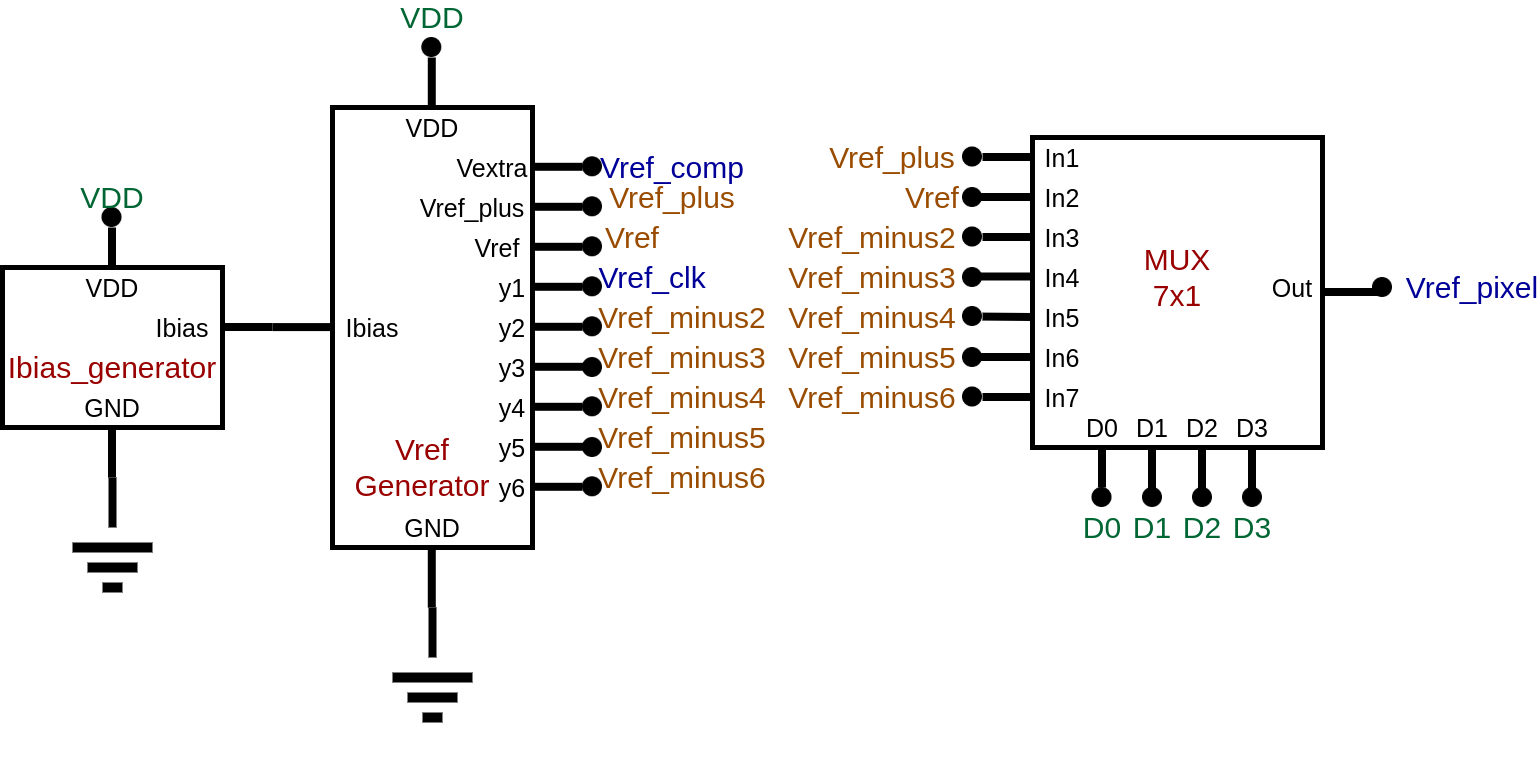
\includegraphics[scale=0.3]{Circuitos/vref_block.png}
    \legend{Fonte: Produzido pelo autor}
\end{figure}

\begin{figure}[htb]
 \centering
    \centering
    \caption{\label{\NomeSFig}Representação em bloco do \NomeBloco}
    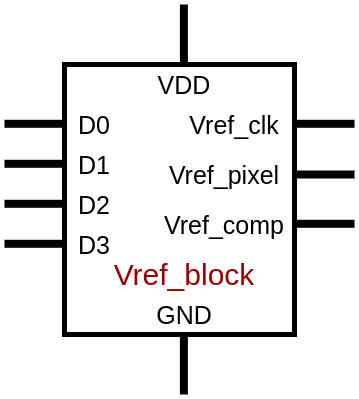
\includegraphics[scale=0.3]{Circuitos/vref_block_block.png}
    \legend{Fonte: Produzido pelo autor}
\end{figure}
\renewcommand{\NomeBloco}{\textit{vref\_block\_with\_mux}}
\renewcommand{\NomeBlocoA}{vrefblockwithmux}
\renewcommand{\NomePTab}{tab_\NomeBlocoA}
\renewcommand{\NomeSTab}{tab_\NomeBlocoA2}
\renewcommand{\NomePFig}{fig_\NomeBlocoA}
\renewcommand{\NomeSFig}{fig_\NomeBlocoA2}
\renewcommand{\NomeTTab}{tab_\NomeBlocoA3}

\section{vref\_block\_with\_mux}

O bloco \NomeBloco{} tem a finalidade de selecionar a tensão de refer\^encia a ser utilizada nos blocos de comparação do circuito, al\'em de retornar a tensão de refer\^encia utilizada pelo bloco \textit{TIA}. A \autoref{\NomePTab} indica a Tabela Verdade do bloco. Embora tenha uma l\'ogica digital, o circuito permite sa\'idas anal\'ogicas.

\begin{table}[!h]

\caption{Tabela Verdade do bloco \NomeBloco}%
\label{\NomePTab}
\centering
\begin{tabular}{ccccc}
    \toprule
    D0 & D1 & D2 & D3 & Out \\
    \midrule \midrule
    0 & 0 & 0 & 0 & Vref\_plus\\
    \midrule
    0 & 1 & 0 & 0 & Vref\\
    \midrule
    1 & 0 & 0 & 0 & Vref\_minus2\\
    \midrule
    1 & 1 & 0 & 0 & Vref\_minus3\\
    \midrule
    X & X & 0 & 1 & Vref\_minus4\\
    \midrule
    X & X & 1 & 0 & Vref\_minus5\\
    \midrule
    X & X & 1 & 1 & Vref\_minus6\\
\bottomrule

\end{tabular}
\fonte{Produzido pelo autor.}
\end{table}

O bloco apresenta as definições de sinais de entrada e sa\'ida referidos na \autoref{\NomeSTab}.

\begin{table}[!h]
\caption{Sinais do bloco \NomeBloco}
\label{\NomeSTab}
\centering
\begin{tabular}{ccl}

    \toprule
    Sinal & Tipo    & Descrição      \\
    \midrule \midrule
    D0   & Entrada   & Entrada de seleção 1 \\
    \midrule
    D1   & Entrada   & Entrada de seleção 2 \\
    \midrule
    D2   & Entrada   & Entrada de seleção 3 \\
    \midrule
    D3   & Entrada   & Entrada de seleção 4 \\
    \midrule
    Vref\_pixel   & Sa\'ida   & Tensão de refer\^encia selecionada \\
    \midrule
    Vref\_clk¹  & Sa\'ida   & Tensão de refer\^encia do Clock \\
    \midrule
    Vref\_comp²  & Sa\'ida   & Tensão de refer\^encia do Clock do bloco teste \\
    \bottomrule
\end{tabular}
\legend{Fonte: Produzido pelo autor}
\legend{¹ Essa tensão \'e igual \'a sa\'ida Vref\_minus do bloco \textit{vref\_block}\\² Essa tensão \'e igual \'a sa\'ida Vref\_extra do bloco \textit{vref\_block}}
\end{table}

O circuito projetado para o bloco \'e demonstrado na \autoref{\NomePFig}.

\begin{figure}[htb]
 \centering
    \centering
    \caption{\label{\NomePFig}Circuito CMOS projetado para o bloco \NomeBloco}
    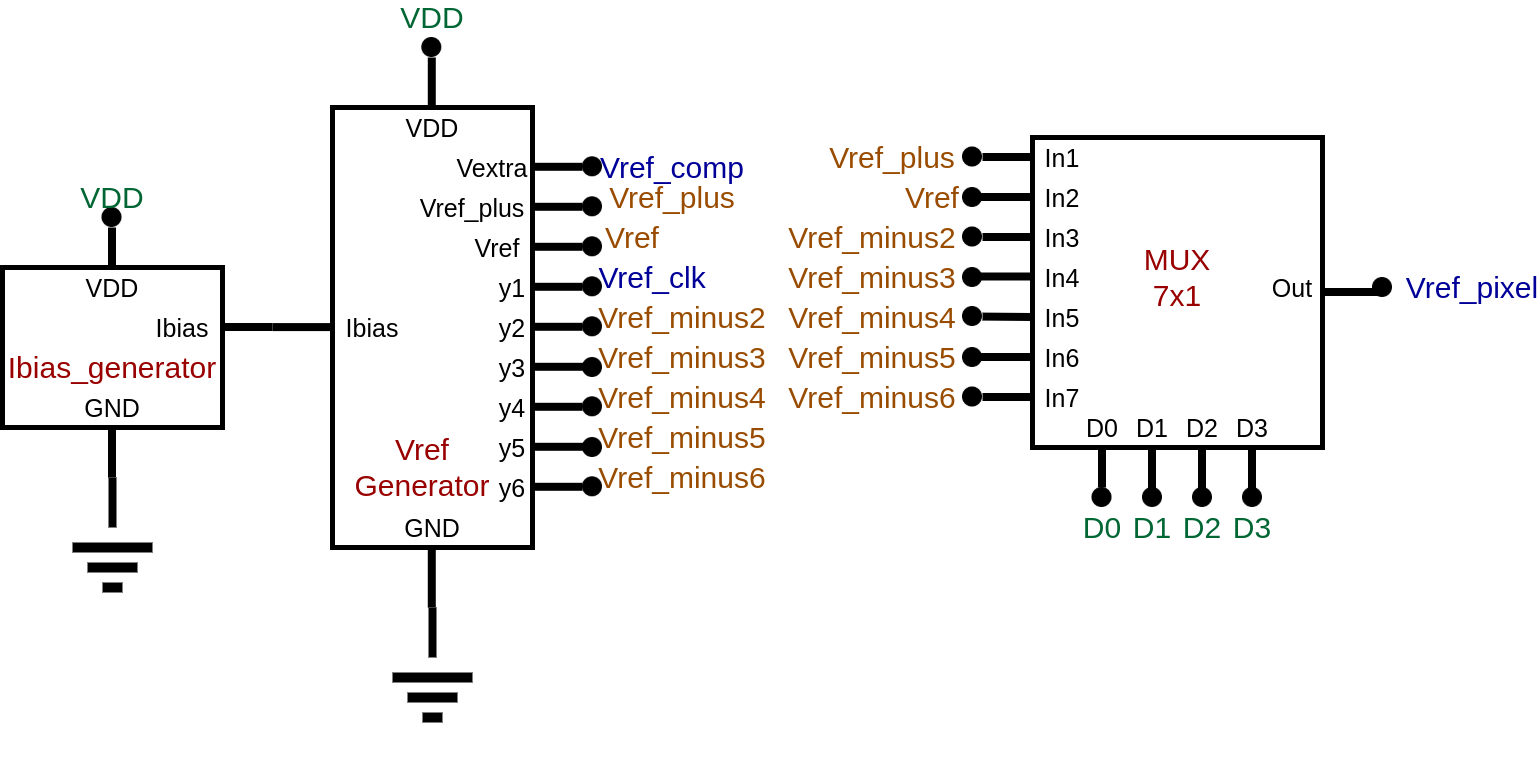
\includegraphics[scale=0.28]{Circuitos/vref_block.png}
    \legend{Fonte: Produzido pelo autor}
\end{figure}

\begin{figure}[htb]
 \centering
    \centering
    \caption{\label{\NomeSFig}Representação em bloco do \NomeBloco}
    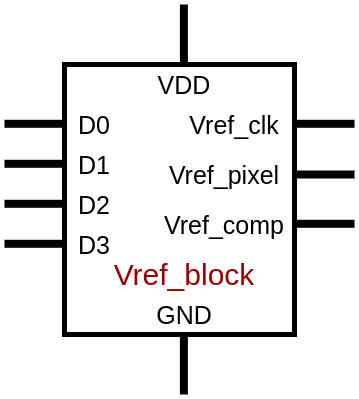
\includegraphics[scale=0.3]{Circuitos/vref_block_block.png}
    \legend{Fonte: Produzido pelo autor}
\end{figure}

\renewcommand{\NomeBloco}{\textit{ibias\_block}}
\renewcommand{\NomeBlocoA}{ibiasblock}
\renewcommand{\NomePTab}{tab_\NomeBlocoA}
\renewcommand{\NomeSTab}{tab_\NomeBlocoA2}
\renewcommand{\NomePFig}{fig_\NomeBlocoA}
\renewcommand{\NomeSFig}{fig_\NomeBlocoA2}
\renewcommand{\NomeTTab}{tab_\NomeBlocoA3}

\section{ibias\_block}

O bloco \NomeBloco{} gera diversos drenos de corrente utilizados por outros blocos. O bloco apresenta as definições de sinais de entrada e sa\'ida referidos na \autoref{\NomeSTab}.

\begin{table}[!h]
\caption{Sinais do bloco \NomeBloco}
\label{\NomeSTab}
\centering
\begin{tabular}{ccl}

    \toprule
    Sinal & Tipo    & Descrição      \\
    \midrule \midrule
    bias\_pixel\_1   & Sa\'ida   & Dreno de corrente para o APS 1 (0,5 $\mu$A) \\
    \midrule
    bias\_pixel\_2   & Sa\'ida   & Dreno de corrente para o APS 2 (0,5 $\mu$A) \\
    \midrule
    bias\_pixel\_3   & Sa\'ida   & Dreno de corrente para o APS 3 (0,5 $\mu$A) \\
    \midrule
    bias\_pixel\_4   & Sa\'ida   & Dreno de corrente para o APS 4 (0,5 $\mu$A) \ \\
    \midrule
    extra\_500nA   & Sa\'ida   & Dreno de corrente para o APS de teste (0,5 $\mu$A) \ \\
    \midrule
    bias\_comp\_1   & Sa\'ida   & Dreno de corrente para o Comparador 1 (1,5 $\mu$A) \ \\
    \midrule
    bias\_comp\_2   & Sa\'ida   & Dreno de corrente para o Comparador 2 (1,5 $\mu$A) \ \\
    \midrule
    bias\_comp\_3   & Sa\'ida   & Dreno de corrente para o Comparador 3 (1,5 $\mu$A) \\
    \midrule
    bias\_comp\_4   & Sa\'ida   & Dreno de corrente para o Comparador 4 (1,5 $\mu$A) \\
    \midrule
    extra\_1500nA   & Sa\'ida   & Dreno de corrente para o Comparador de teste (1,5 $\mu$A) \ \\
    \bottomrule
\end{tabular}
\legend{Fonte: Produzido pelo autor}
\legend{¹ Essa tensão \'e igual a sa\'ida Vref\_minus do bloco \textit{vref\_block}\\² Essa tensão \'e igual a sa\'ida Vref\_extra do bloco \textit{vref\_block}}
\end{table}

O circuito projetado para o bloco \'e demonstrado na \autoref{\NomePFig}.

\begin{figure}[!h]
 \centering
    \centering
    \caption{\label{\NomePFig}Circuito CMOS projetado para o bloco \NomeBloco} 
    \includegraphics[scale=0.3]{Circuitos/ibias_block.png}
    \legend{Fonte: Produzido pelo autor}
\end{figure}


\begin{figure}[!h]
 \centering
    \centering
    \caption{\label{\NomeSFig}Representação em bloco do \NomeBloco}
    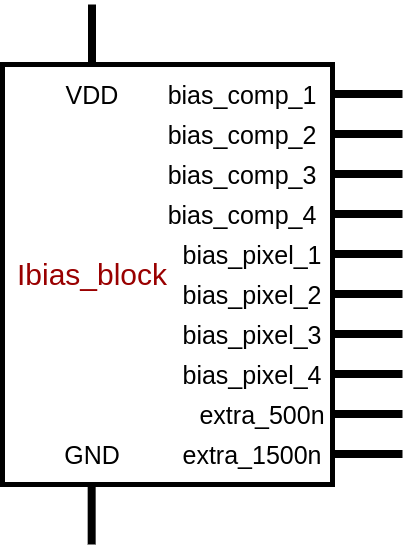
\includegraphics[scale=0.3]{Circuitos/ibias_block_block.png}
    \legend{Fonte: Produzido pelo autor}
\end{figure}
\clearpage

\renewcommand{\NomeBloco}{\textit{APS\_3}}
\renewcommand{\NomeBlocoNoUnderline}{apsthree}
\renewcommand{\NomePTab}{tab_\NomeBlocoNoUnderline}
\renewcommand{\NomeSTab}{tab_\NomeBlocoNoUnderline2}
\renewcommand{\NomePFig}{fig_\NomeBlocoNoUnderline}
\renewcommand{\NomeSFig}{fig_\NomeBlocoNoUnderline2}
\renewcommand{\NomeTTab}{tab_\NomeBlocoNoUnderline3}
\renewcommand{\NomeQTab}{tab_\NomeBlocoNoUnderline4}

\section{APS\_3}

O \textit{\NomeBloco} \'e o circuito respons\'avel por armazenar todos os tr\^es blocos APS de cor (Azul, Verde, Vermelho), mais o TIA geradora de rel\'ogio de refer\^encia para os APS's citados. O bloco apresenta as definicões de sa\'ida referidos na \autoref{\NomeSTab}.

As sa\'idas digitais de cada bloco APS\_3 apresentam um buffer, de forma a garantir a integridade do sinal nos pinos do Circuito Integrado.

\begin{figure}[!h]
 \centering
    \centering
    \caption{\label{\NomeSFig}Representacão em bloco do \NomeBloco}
    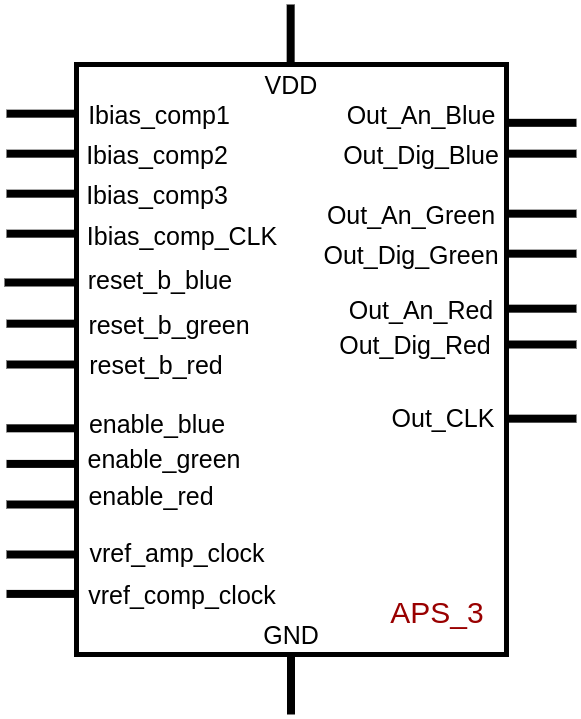
\includegraphics[scale=0.3]{Circuitos/APS_3_block.png}
    \legend{Fonte: Produzido pelo autor}
\end{figure}

\begin{table}[!h]
\centering
  \caption{Descricão dos sinais de entrada e sa\'ida do circuito projetado para as cores azul, verde e vermelha}%
  \label{\NomeSTab}
  \begin{tabular}{ccll}
  \toprule
   Sinal & Tipo & Descricão & Observacão \\
  \midrule \midrule
   RESET\_BLUE & Entrada & \begin{tabular}[l]{@{}l@{}}Sinal de tensão \textit{RESET}\\ no APS para cor azul\end{tabular} & Ativo em n\'ivel baixo \\
  \midrule
   RESET\_GREEN & Entrada & \begin{tabular}[l]{@{}l@{}}Sinal de tensão de \textit{RESET}\\ no APS para cor verde\end{tabular} & Ativo em n\'ivel baixo \\
  \midrule
   RESET\_RED & Entrada & \begin{tabular}[l]{@{}l@{}}Sinal de tensão \textit{RESET}\\ no APS para cor vermelha\end{tabular} & Ativo em n\'ivel baixo \\
   \midrule
   ENABLE\_BLUE & Entrada & \begin{tabular}[l]{@{}l@{}}Sinal de tensão \textit{ENABLE} \\no APS para cor azul\end{tabular} & Ativo em n\'ivel alto \\
  \midrule
   ENABLE\_GREEN & Entrada & \begin{tabular}[l]{@{}l@{}}Sinal de tensão \textit{ENABLE} \\no APS para cor verde\end{tabular} & Ativo em n\'ivel alto \\
  \midrule
   ENABLE\_RED & Entrada & \begin{tabular}[l]{@{}l@{}}Sinal de tensão \textit{ENABLE}\\ no APS para cor vermelha\end{tabular} & Ativo em n\'ivel alto \\
  \midrule
   Ibias\_comp1 & Entrada & \begin{tabular}[l]{@{}l@{}}Fonte de corrente para\\ cor Azul\end{tabular} &  \\
   \midrule
   Ibias\_comp2 & Entrada & \begin{tabular}[l]{@{}l@{}}Fonte de corrente para\\ cor Verde\end{tabular} &  \\
   \midrule
   Ibias\_comp3 & Entrada & \begin{tabular}[l]{@{}l@{}}Fonte de corrente para\\ cor Vermelha\end{tabular} &  \\
   \midrule
   Ibias\_clk & Entrada & \begin{tabular}[l]{@{}l@{}}Fonte de corrente para o\\ bloco \textit{APS\_pixel\_clk}\end{tabular}
    &  \\
  \midrule
   Out\_An\_Blue & Sa\'ida & \begin{tabular}[l]{@{}l@{}}Sinal anal\'ogico para cor\\ azul\end{tabular} \\
  \midrule
   Out\_Dig\_Blue & Sa\'ida & Sinal digital para cor azul \\
  \midrule
   Out\_An\_Green & Sa\'ida & \begin{tabular}[l]{@{}l@{}}Sinal anal\'ogico para cor\\ verde\end{tabular} \\
  \midrule
   Out\_Dig\_Green & Sa\'ida & Sinal digital para cor verde \\
  \midrule
   Out\_An\_Red & Sa\'ida & \begin{tabular}[l]{@{}l@{}}Sinal anal\'ogico para cor\\ vermelha\end{tabular} \\
  \midrule
   Out\_Dig\_Red & Sa\'ida & \begin{tabular}[l]{@{}l@{}}Sinal digital para cor\\ vermelha\end{tabular} \\
  \bottomrule
  \end{tabular}
  \legend{Fonte: Produzido pelo autor.}
\end{table}

O circuito projetado para o bloco \'e demonstrado na \autoref{\NomePFig}.

\clearpage

\begin{figure}[!h]
 \centering
    \centering
    \caption{Circuito CMOS projetado para o bloco \NomeBloco} 
    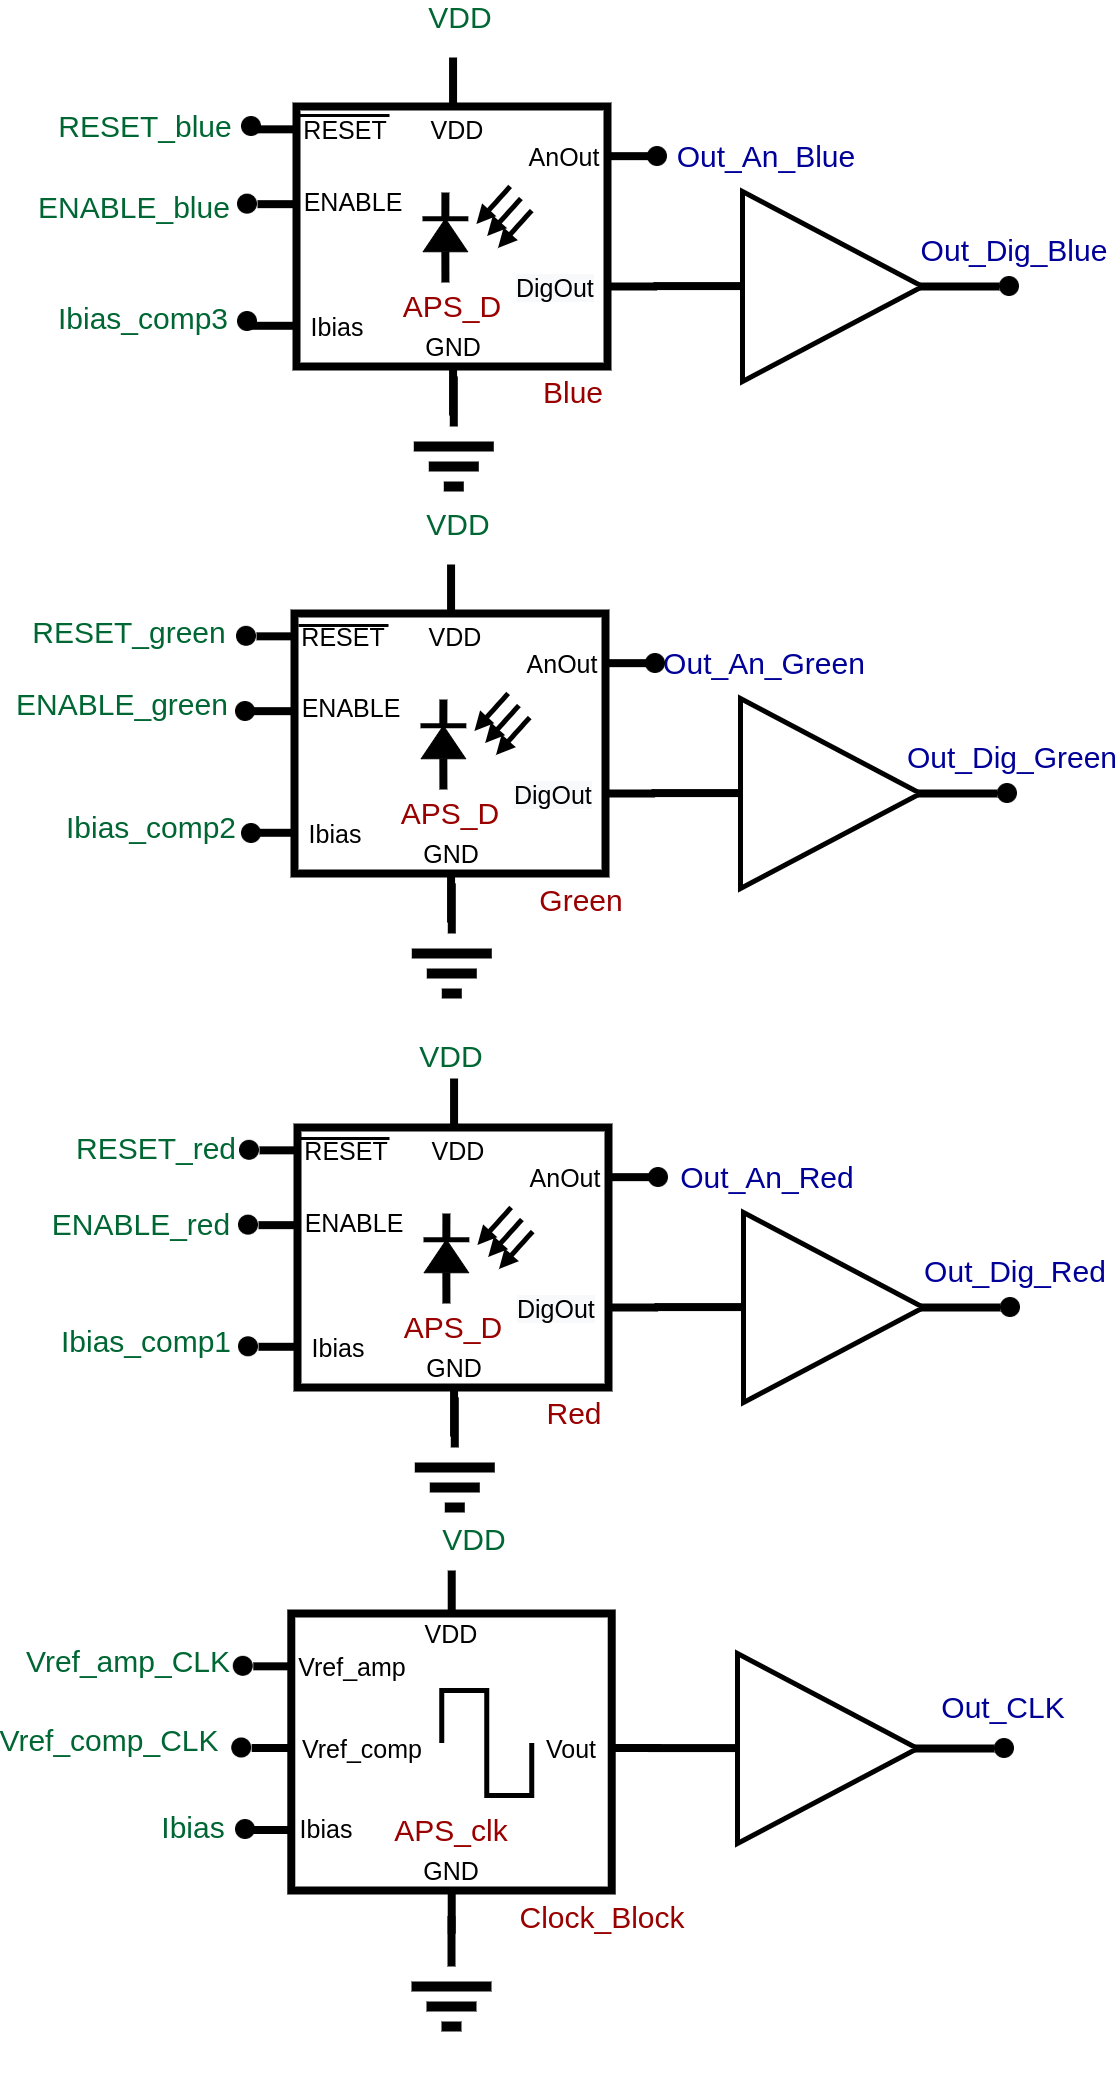
\includegraphics[scale=0.3]{Circuitos/APS_3.png}
    \legend{Fonte: Produzido pelo autor}
    \label{\NomePFig}
\end{figure}
\renewcommand{\NomeBloco}{\textit{Comparador}}
\renewcommand{\NomeBlocoNoIt}{Comparador}
\renewcommand{\NomePTab}{tab_\NomeBloco}
\renewcommand{\NomeSTab}{tab_\NomeBlocoNoIt2}
\renewcommand{\NomePFig}{fig_\NomeBlocoNoIt}
\renewcommand{\NomeSFig}{fig_\NomeBlocoNoIt2}
\renewcommand{\NomeTTab}{tab_\NomeBlocoNoIt3}

\section{Comparador}

O bloco \NomeBloco{} tem a função de comparar dois sinais anal\'ogicos advindos nas entradas '+' (\textit{Vp}) e '-' (\textit{Vn}), e retornar \textit{VDD} caso Vp seja maior do que Vn, e \textit{GND} caso Vp seja menor ou igual a Vn. O bloco apresenta as definições de sinais de entrada e sa\'ida referidos na \autoref{\NomeSTab}.

\begin{table}[!h]
\caption{Sinais do bloco \NomeBloco}
\label{\NomeSTab}
\centering
\begin{tabular}{ccl}

    \toprule
    Sinal & Tipo    & Descrição        \\
    \midrule \midrule
    Vp (+) & Entrada & Entrada positiva do Comparador\\
    \midrule
    Vn (-) & Entrada & Entrada negativa do Comparador\\
    \midrule
    Ibias & Entrada & Corrente de polarização do Comparador\\
    \midrule
    Vo & Sa\'ida & Sa\'ida do Comparador\\
    \bottomrule
\end{tabular}
\legend{Fonte: Produzido pelo autor}
\end{table}

O circuito projetado para o bloco \'e demonstrado na \autoref{\NomePFig}.

\begin{figure}[!h]
 \centering
    \centering
    \caption{Circuito CMOS projetado para o bloco \NomeBloco} 
    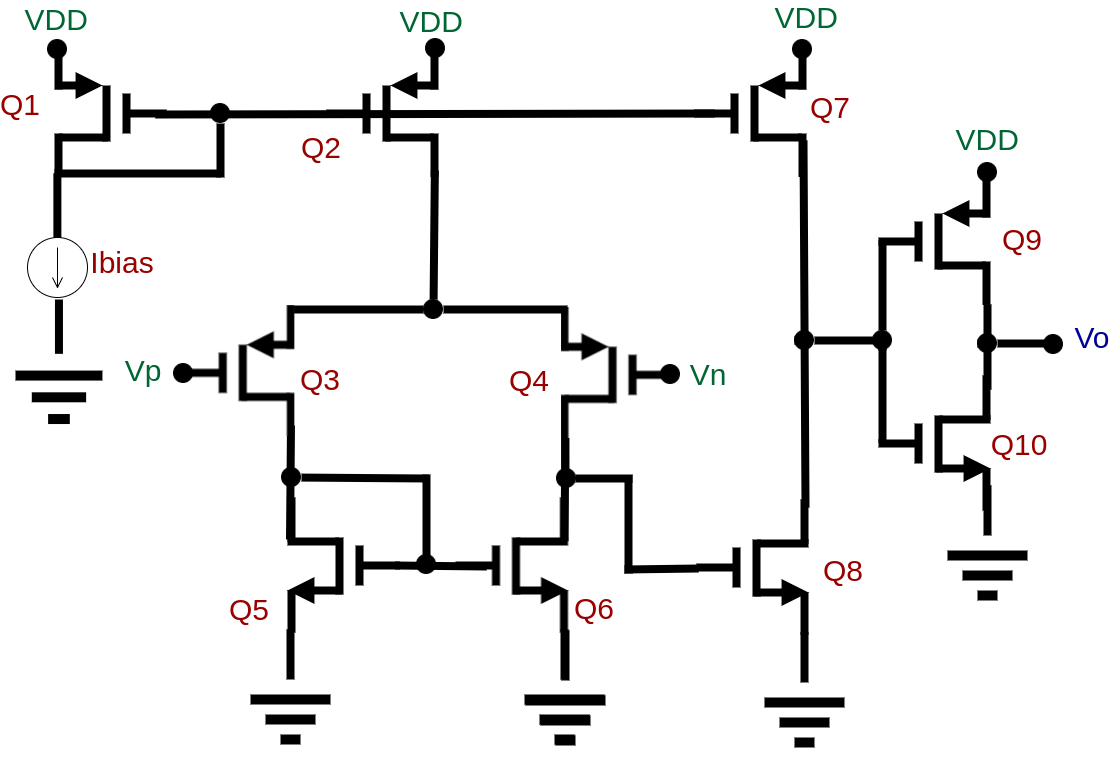
\includegraphics[scale=0.3]{Circuitos/Comparator.png}
    \legend{Fonte: Produzido pelo autor}
    \label{\NomePFig}
\end{figure}

\begin{figure}[!h]
 \centering
    \centering
    \caption{\label{\NomeSFig}Representação em bloco do \NomeBloco}
    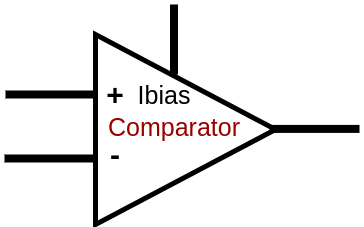
\includegraphics[scale=0.3]{Circuitos/Comparator_block.png}
    \legend{Fonte: Produzido pelo autor}
\end{figure}

Os transistores utilizados no bloco \NomeBloco{} apresentam os par\^ametros mostrados na \autoref{\NomeTTab}.

\begin{table}[!h]
\caption{Transistores do Bloco \NomeBloco}
\label{\NomeTTab}
\centering
\begin{tabular}{ccccc}
\toprule
Transistor & W ($\mu$m)  & L ($\mu$m)           & M (n° dispositivos) & S (n° dispositivos)\\
\midrule \midrule
Q1 & 10 & 1 & 1 & 1\\
\midrule
Q2$^1$ & 10 & 1 & 6 & 6\\
\midrule
Q3 & 4 & 1 & 2 & 2\\
\midrule
Q4 & 4 & 1 & 2 & 2\\
\midrule
Q5 & 2 & 1 & 2 & 2\\
\midrule
Q6 & 2 & 1 & 2 & 2\\
\midrule
Q7$^1$ & 10 & 1 & 8 & 8\\
\midrule
Q8 & 2 & 1 & 4 & 4\\
\midrule
Q9 & 3 & 0.18 & 1 & 1\\
\midrule
Q10 & 1.5 & 0.18 & 1 & 1\\

\bottomrule
\end{tabular}
\legend{Fonte: Produzido pelo autor}
\legend{$^1$Calculado de forma a produzir uma corrente de 9 $\mu$A}
\end{table}
 
O \NomeBloco{} \'e desenvolvido com dois est\'agios de amplificação. O primeiro est\'agio, composto pelos transistores Q3, Q4, Q5, Q6 t\^em a função de realizar a diferença entra as entradas \textit{Vp} e \textit{Vn} e multiplicar por um pequeno ganho. Os transistores Q3 e Q4 são respons\'aveis por receber as entradas, enquanto os transistores Q5 e Q6 funcionam como transistores de Carga Ativa. O Q2 funciona como uma fonte de corrente.

O segundo est\'agio \'e um est\'agio de ganho, do qual o transistor Q2 fornece um ganho para a saía do est\'agio anterior e o transistor Q7 funciona como uma fonte de corrente para o est\'agio.

Diodos quadrados \textit{D1} e \textit{D2} de proteção são inclu\'idos nos terminais \textit{Vp} e \textit{Vn do circuito}, com \^anodo ligado ao terra e catodo ligado ao seu respectivo terminal. Os diodos apresentam os seguintes par\^ametros apresentados na \autoref{diodosComp}.

\begin{table}[!h]
\caption{Diodos do Bloco \NomeBloco}
\label{diodosComp}
\centering
\begin{tabular}{cccc}
\toprule
Diodo & W ($\mu$m)  & L ($\mu$m)           & \'Area ($\mu$m²)\\
\midrule \midrule
D1 e D2 & 1 & 1 & 1 \\

\bottomrule
\end{tabular}
\legend{Fonte: Produzido pelo autor}
\end{table}

\section{Circuitos de Teste}
\label{BlocoTestes}

O circuito apresenta dois circuitos de teste adicionais, sendo um para um APS e outro para o TIA. A finalidade destes circuitos \'e de testar o sistema sem a necessidade de uma fonte luminosa. Para isso \'e acrescentado um pino diretamente aos catodos dos fotodiodos, em que uma tensão pode ser diretamente injetada nos mesmos de forma a simular a fotogeração.

O APS de teste utiliza os pinos de RESET e ENABLE iguais ao do APS de cor azul, mas \'e polarizado com uma fonte de corrente pr\'opria e também apresenda sa\'idas pr\'oprias. Caso se mantenha o pino de injeção de corrente flutuante, o APS deve funcionar de forma equivalente aos outros.
\section{Layout}

Com todos os blocos definidos e o esquemático elétrico desenvolvido, foi possível iniciar o desenvolvimento do layout. Todo o projeto foi realizado utilizando a ferramenta \textit{Virtuoso}, da \textit{Cadence}, utilizando o processo \textit{TSMC CMOS 180 nm}.

A \autoref{layoutcompleto} apresenta a implementação completa do Receptor Óptico projetado. A \autoref{layoutcompleto_division} mostra a mesma figura explicitando o que representa as diferentes partes do circuito. O projeto do Receptor Óptico ocupa uma área total de 633,9x666,96 $\mu$m\textsuperscript{2} ($\approx$~0,423 mm\textsuperscript{2}).

Alguns dos blocos auxiliares do receptor foram desenvolvidos por \textit{Felipe Magalhães} (autor deste trabalho) e \textit{Daniel Carvalho Lott} em seus projetos de Iniciação Cientifica. Os layouts desses blocos estão apresentados de maneira implícita junto aos circuitos apresentados ao longo de todo capítulo.

\begin{figure}[!h]
 \centering
    \caption{Layout completo do circuito desenvolvido} 
    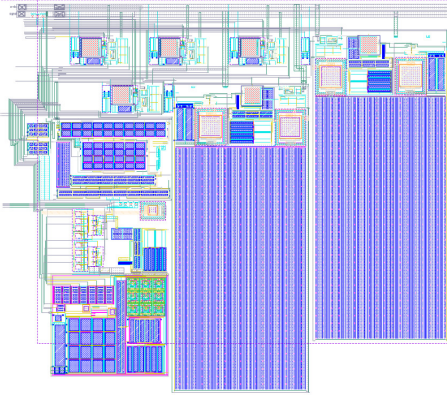
\includegraphics[scale=1, angle = 90]{Projeto/Layout/Imagens/Circuito Completo.png}
    \legend{Fonte: Produzido pelo autor}
    \label{layoutcompleto}
    \nota{Imagem rotacionada em 90° em sentido anti-horário}
\end{figure}

\begin{figure}[!h]
 \centering
    \caption{Layout completo do circuito particionado} 
    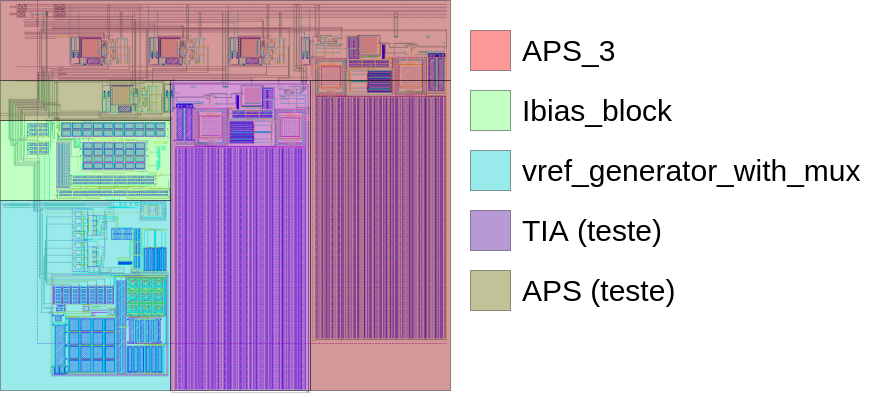
\includegraphics[scale=0.4]{Projeto/Layout/Imagens/Image_CircuitoCompleto.png}
    \legend{Fonte: Produzido pelo autor}
    \label{layoutcompleto_division}
\end{figure}

O bloco \textit{APS\_digitalized} projetado é apresentado na figura \autoref{layoutAPSDIG}. A \autoref{layoutAPSDIG_division} mostra a mesma figura explicitando o que representa as diferentes parte do circuito. O projeto do bloco ocupa uma área total aproximada de 3307 $\mu$m\textsuperscript{2}.

\begin{figure}[!h]
 \centering
    \centering
    \caption{Layout do bloco \textit{APS\_digitalized}} 
    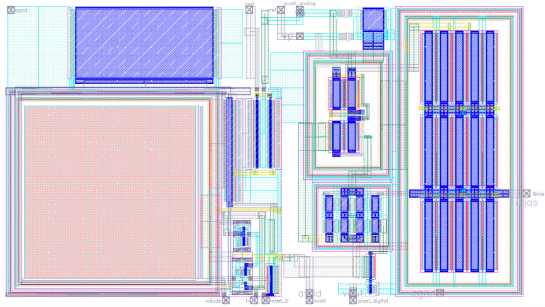
\includegraphics[scale=0.8]{Projeto/Layout/Imagens/APS_DIGITALIZED.png}
    \legend{Fonte: Produzido pelo autor}
    \label{layoutAPSDIG}
\end{figure}

\begin{figure}[!h]
 \centering
    \centering
    \caption{Layout do bloco \textit{APS\_digitalized} particionado} 
    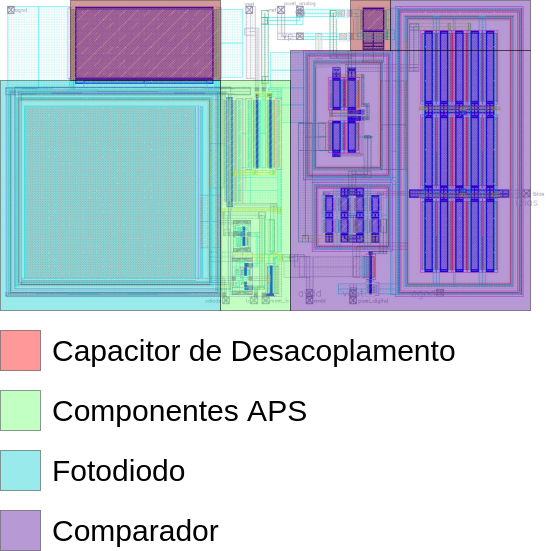
\includegraphics[scale=0.3]{Projeto/Layout/Imagens/Image_APS_Digitalized.png}
    \legend{Fonte: Produzido pelo autor}
    \label{layoutAPSDIG_division}
\end{figure}

O bloco \textit{APS\_clk} projetado é apresentado na figura \autoref{layoutTIA}. A \autoref{layoutTIA_division} mostra a mesma figura explicitando o que representa as diferentes parte do circuito. O projeto do bloco ocupa uma área total aproximada de 102107 um\textsuperscript{2}.

\begin{figure}[!h]
 \centering
    \begin{minipage}{0.5\textwidth}
    \centering
    \caption{Layout do bloco \textit{APS\_clk}} 
    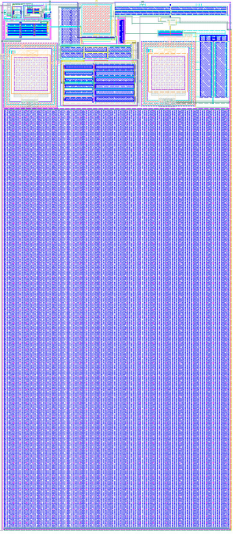
\includegraphics[scale=0.7]{Projeto/Layout/Imagens/TIA.png}
    \legend{Fonte: Produzido pelo autor}
    \label{layoutTIA}
    \end{minipage}
    \hfill
    \begin{minipage}{0.4\textwidth}
    \centering
    \caption{Layout do bloco \textit{APS\_clk} particionado}
    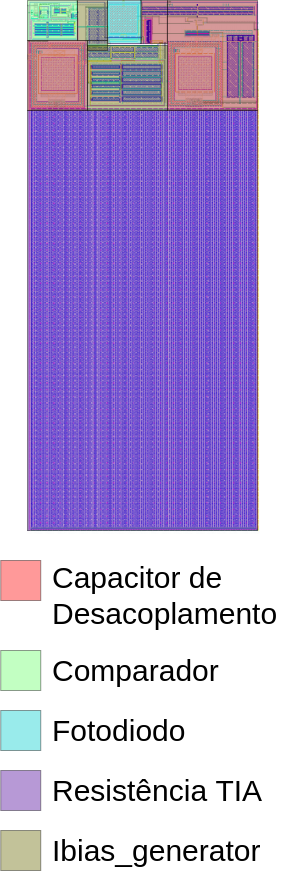
\includegraphics[scale=0.4]{Projeto/Layout/Imagens/Image_TIA.png}
    \legend{Fonte: Produzido pelo autor}
    \label{layoutTIA_division}
    \end{minipage}
\end{figure}

O bloco \textit{APS\_3} projetado é apresentado na figura \autoref{layoutAPS_3}. A \autoref{layoutAPS_3_division} mostra a mesma figura explicitando o que representa as diferentes parte do circuito. O projeto do bloco ocupa uma área aproximada de 123353 $\mu$m\textsuperscript{2}.

\begin{figure}[!h]
    \centering
    \caption{Layout do bloco \textit{APS\_3}} 
    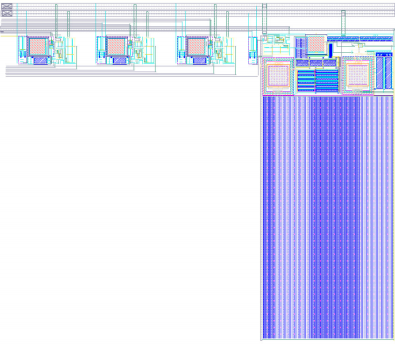
\includegraphics[scale=1]{Projeto/Layout/Imagens/APS_3.png}
    \legend{Fonte: Produzido pelo autor}
    \label{layoutAPS_3}
\end{figure}

\begin{figure}[!h]
    \centering
    \caption{Layout do bloco \textit{APS\_3} particionado} 
    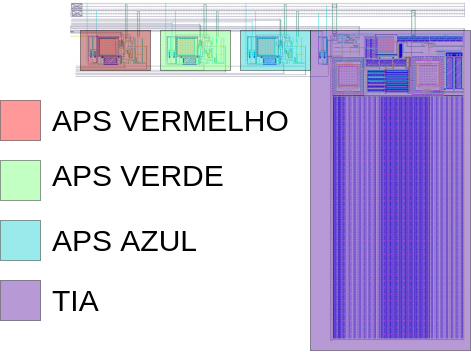
\includegraphics[scale=0.4]{Projeto/Layout/Imagens/Image_APS_3.png}
    \legend{Fonte: Produzido pelo autor}
    \label{layoutAPS_3_division}
\end{figure}

\clearpage

\section{Chip}

O circuito integrado apresentado na \autoref{fig_circintegrado} foi desenvolvido, contendo todo o projeto de Receptor Óptico além de outros projetos desenvolvidos por terceiros. A \autoref{fig_circintegrado_division} mostra de maneira explicita o que representa cada parte do CI, e referências aos outros projetos desenvolvidos.

O circuito integrado apresenta uma área total de 1,6x1,6 mm\textsuperscript{2} (2,56 mm\textsuperscript{2}), utilizando um encapsulamento do tipo CLCC44\footnote{Especificações do encapsulamento presentes no \autoref{anexo_clcc44}}. A \autoref{tab_clcc44} apresenta a relação da numeração dos pinos do encapsulamento com os pinos chip, que são distintos, além da identificação de cada pino.

Diversos capacitores de desacoplamento foram incluídos ao longo de todo chip, com o objetivo de preencher áreas não utilizadas e também filtrar ruídos apresentados nos sinais das fontes de alimentação que chegam e percorrem o chip. 

\begin{figure}[!h]
 \centering
    \caption{Circuito Integrado utilizado para o Receptor Óptico} 
    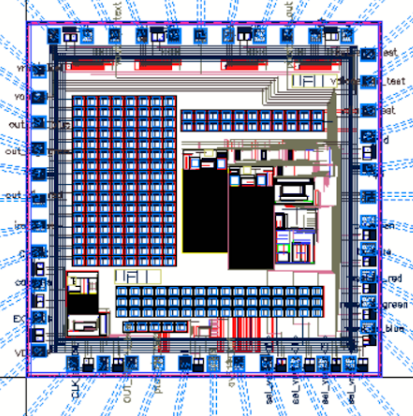
\includegraphics[scale=0.5]{Projeto/Layout/Imagens/CircuitoIntegrado.png}
    \legend{Fonte: Produzido pelo autor}
    \label{fig_circintegrado}
\end{figure}

\begin{figure}[!h]
 \centering
    \caption{Circuito Integrado utilizado para o Receptor Óptico particionado} 
    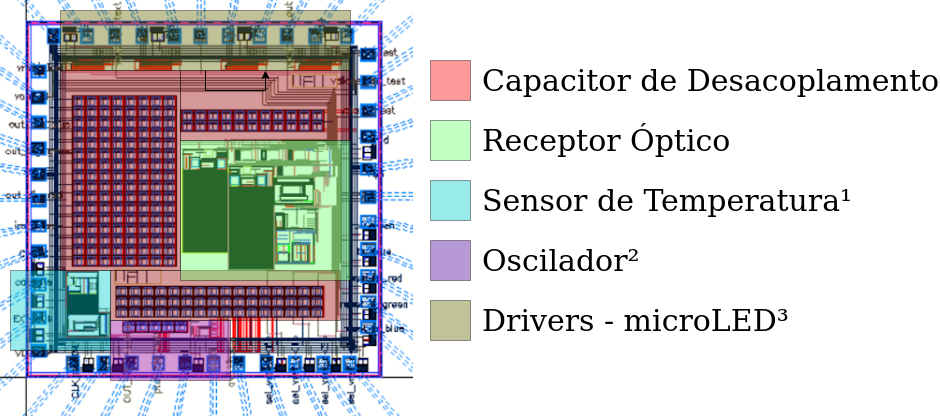
\includegraphics[scale=0.4]{Projeto/Layout/Imagens/Image_CircuitoIntegrado.png}
    \legend{Fonte: Roteamento de top-level realizados por Prof. Hugo, Daniel Lott e Prof. Dalton}
    \label{fig_circintegrado_division}
    \nota{\textsuperscript{1} Trabalho de Conclusão de Curso de Daniel Carvalho Lott \cite{DanielLott}\\\textsuperscript{2} Trabalho de Conclusão de Curso de Victor Rodrigues Barbosa \cite{VictorRodrigues}\\\textsuperscript{3} Trabalho realizado pelo aluno de Mestrado Rubens Alcântara de Souza, da UFMG}
\end{figure}

\begin{table}[!h]
\caption{Pinos presentes no circuito integrado para o Receptor Óptico}
\footnotesize
\begin{tabular}{cccll}
\toprule
\begin{tabular}[c]{@{}c@{}}Pino\\ Circuito \\ Integrado\end{tabular} & \begin{tabular}[c]{@{}c@{}}Pino\\ Chip\end{tabular} & Nome              & \multicolumn{1}{c}{Descrição}                                                                           & \multicolumn{1}{c}{Observação}                                                                                           \\
\midrule \midrule
1                                                                 & 40                                                  & vref\_pixel       & Não utilizado                                                                    &                                \\\midrule
2                                                                 & 41                                                  & vout\_clk         & Tensão de saída de relógio gerada                                                                       &                                \\\midrule
3                                                                 & 42                                                  & out\_dig\_blue    & \begin{tabular}[c]{@{}l@{}}Sinal de tensão digital\\ para cor azul\end{tabular}                         &                                \\\midrule
4                                                                 & 43                                                  & out\_dig\_green   & \begin{tabular}[c]{@{}l@{}}Sinal de tensão digital\\ para cor verde\end{tabular}                        &                                \\\midrule
5                                                                 & 44                                                  & VSS               & Terra                                                                                                   &                                \\\midrule
6                                                                 & 1                                                   & out\_dig\_red     & \begin{tabular}[c]{@{}l@{}}Sinal de tensão digital\\ para cor vermelha\end{tabular}                     &                                \\\midrule
7                                                                 & 2                                                   & iref\_test        & Não utilizado                                                                        &                                \\\midrule
23                                                                & 18                                                  & reset\_b\_blue    & \begin{tabular}[c]{@{}l@{}}Sinal de tensão de RESET\\ no APS para cor azul\end{tabular}                 & Ativo em nível baixo           \\\midrule
24                                                                & 19                                                  & reset\_b\_green   & \begin{tabular}[c]{@{}l@{}}Sinal de tensão de RESET\\ no APS para cor verde\end{tabular}                & Ativo em nível baixo           \\\midrule
25                                                                & 20                                                  & reset\_b\_red     & \begin{tabular}[c]{@{}l@{}}Sinal de tensão de RESET\\ no APS para cor vermelha\end{tabular}             & Ativo em nível baixo           \\\midrule
26                                                                & 21                                                  & tx\_blue          & \begin{tabular}[c]{@{}l@{}}Sinal de tensão de ENABLE\\ no APS para cor azul\end{tabular}                & Ativo em nível alto            \\\midrule
27                                                                & 22                                                  & tx\_green         & \begin{tabular}[c]{@{}l@{}}Sinal de tensão de ENABLE\\ no APS para cor verde\end{tabular}               & Ativo em nível alto            \\\midrule
28                                                                & 23                                                  & V18               & Tensão de alimentação de 1,8V                                                                           &                                \\\midrule
29                                                                & 24                                                  & VSS               & Terra                                                                                                   &                                \\\midrule
30                                                                & 25                                                  & tx\_red           & \begin{tabular}[c]{@{}l@{}}Sinal de tensão de ENABLE\\ no APS para cor vermelha\end{tabular}            & Ativo em nível alto            \\\midrule
31                                                                & 26                                                  & vdiode\_test      & \begin{tabular}[c]{@{}l@{}}Corrente que simula fotogeração\\ no APS de teste\end{tabular} &                                \\\midrule
32                                                                & 27                                                  & vdiode\_clk\_test & \begin{tabular}[c]{@{}l@{}}Corrente que simula fotogeração\\ no fotodiodo no TIA de teste\end{tabular} &                                \\\midrule
33                                                                & 28                                                  & out\_ana\_test    & \begin{tabular}[c]{@{}l@{}}Sinal de tensão analógico para o\\ APS de teste\end{tabular}                 &         \\\bottomrule                      
\end{tabular}
\label{tab_clcc44}
\legend{Fonte: Produzido pelo autor}
\end{table}
